\documentclass[tocnosub,noragright,centerchapter,12pt]{uiucecethesis09}

% Use draftthesis for notes and date markings on every page.  Useful when you
%   have multiple copies floating around.
% Use offcenter for the extra .5 inch on the left side. Needed with fullpage and fancy.
% Use mixcasechap for compatibility with hyperref package, which does NOT like all caps default
% Use edeposit for the adviser/committee on the title page.
% Use tocnosub to suppress subsection and lower entries in the TOC.
% PhD candidates use "proquest" for the proquest abstract.

\makeatletter

\usepackage{setspace}
\usepackage{epsfig}  % for figures
\usepackage{xcolor}
%\usepackage{subfigure}  % for subfigures
\usepackage{mathtools}
\usepackage{cancel}  % for cancelling math terms
\usepackage{lscape}  % Useful for wide tables or figures.
\usepackage{bm}
\usepackage[justification=raggedright]{caption}	% makes captions ragged right - thanks to Bryce Lobdell
\usepackage{easy-todo}

\msthesis

\title{Subpixel Multiframe Registration for Formation Flying Spacecraft}
\author{Evan Widloski}
\department{Electrical and Computer Engineering}
\degreeyear{2020}

\advisor{Professor Farzad Kamalabadi}

% Uncomment the \committee command for
% - all doctoral students
% - master's students who have a master's committee
%\committee{Professor Firstname Lastname, Chair\\
%        Professor Firstname Lastname} % etc.

\begin{document}

\definecolor{red}{HTML}{ef2929}
\definecolor{green}{HTML}{8ae234}
\definecolor{blue}{HTML}{729fcf}
\newcommand{\green}[1]{{\color{green}#1}}
\newcommand{\red}[1]{{\color{red}#1}}
\newcommand{\blue}[1]{{\color{blue}#1}}
\newcommand{\svar}[1]{{(\text{#1})}}
\newcommand{\eqcomment}[1]{\parbox[c]{0.4\linewidth}{\color{gray}#1}}
\newcommand{\eqlinecomment}[1]{\hphantom{{}={}}\parbox{\linewidth}{\color{gray}#1}}
\newcommand{\ip}[2]{\left\langle #1,\,#2 \right\rangle}
\allowdisplaybreaks


%%%%%%%%%%%%%%%%%%%%%%%%%%%%%%%%%%%%%%%%%%%%%%%%%%%%%%%%%%%%%%%%%%%%%%%%%%%%%%%
% COPYRIGHT
%
%\copyrightpage
%\blankpage

%%%%%%%%%%%%%%%%%%%%%%%%%%%%%%%%%%%%%%%%%%%%%%%%%%%%%%%%%%%%%%%%%%%%%%%%%%%%%%%
% TITLE
%
\maketitle

%\raggedright
\parindent 1em%

\frontmatter

%%%%%%%%%%%%%%%%%%%%%%%%%%%%%%%%%%%%%%%%%%%%%%%%%%%%%%%%%%%%%%%%%%%%%%%%%%%%%%%
% ABSTRACT
%

%% \listoftodos

\begin{abstract}
  This thesis develops a multiframe image registration algorithm to accurately estimate the motion parameters of a sequence of images with constant linear translation between frames.  The algorithm is developed with formation flying applications in mind, where such motion is common.  The algorithm is non-iterative (obtaining a registration estimate in a fixed amount of time), efficient (requiring only FFT and spatial scaling operations), and parameterless (requiring no tuning for image classes).  Additionally, the algorithm performs well under extreme levels of noise, obtaining an accurate motion estimate even when individual frames are so severely degraded that high-frequency structures are no longer visible in the individual frames.  The algorithm is tested against synthetic noisy frames which have been generated by a computational pipeline designed to simulate observations that will be made by the \emph{VIrtual Super-resolution Optics with Reconfigurable Swarms} (VISORS) cubesat mission, set to be launched in 2023.
\end{abstract}


%%%%%%%%%%%%%%%%%%%%%%%%%%%%%%%%%%%%%%%%%%%%%%%%%%%%%%%%%%%%%%%%%%%%%%%%%%%%%%%
% DEDICATION
%
\begin{dedication}
% Whatever dedication you want.
To my parents, for their love and support.
\end{dedication}

%%%%%%%%%%%%%%%%%%%%%%%%%%%%%%%%%%%%%%%%%%%%%%%%%%%%%%%%%%%%%%%%%%%%%%%%%%%%%%%
% ACKNOWLEDGMENTS
%
% Put acknowledgments in a file called "ack.tex" and it'll be inputted here.
\begin{acknowledgments}
%% \input{ack}
\end{acknowledgments}

%%%%%%%%%%%%%%%%%%%%%%%%%%%%%%%%%%%%%%%%%%%%%%%%%%%%%%%%%%%%%%%%%%%%%%%%%%%%%%%
% TABLE OF CONTENTS
%
\tableofcontents

%%%%%%%%%%%%%%%%%%%%%%%%%%%%%%%%%%%%%%%%%%%%%%%%%%%%%%%%%%%%%%%%%%%%%%%%%%%%%%%
% LIST OF TABLES
%
% The List of Tables is not strictly necessary. Omitting the List of Tables will
% simplify the thesis check and reduce the number of corrections.
%% \listoftables

%%%%%%%%%%%%%%%%%%%%%%%%%%%%%%%%%%%%%%%%%%%%%%%%%%%%%%%%%%%%%%%%%%%%%%%%%%%%%%%
% LIST OF FIGURES
%
% The List of Figures is not strictly necessary. Omitting the List of Figures will
% simplify the thesis check and reduce the number of corrections.
%% \listoffigures

%%%%%%%%%%%%%%%%%%%%%%%%%%%%%%%%%%%%%%%%%%%%%%%%%%%%%%%%%%%%%%%%%%%%%%%%%%%%%%%
% LIST OF ABBREVIATIONS
%
% The List of Abbreviations is not strictly necessary.
\chapter{List of Symbols and Abbreviations}

\begin{symbollist*}
  \item[ADC] analog to digital converter
  \item[AIA] Atmospheric Imaging Assembly
  \item[ASE] absolute sum of errors
  \item[CMOS] complementary metal-oxide semiconductor
  \item[CPSD] cross power spectral density
  \item[DSC] detector spacecraft
  \item[EBTEL] Enthalpy-based Thermal Evolution of Loops
  \item[EUV] extreme ultraviolet
  \item[FFT] fast Fourier transform
  \item[FOV] field of view
  \item[IDFT] inverse discrete Fourier transform
  \item[IFFT] inverse fast Fourier transform
  \item[NCC] normalized cross correlation
  \item[OSC] optics spacecraft
  \item[PSF] point spread function
  \item[RANSAC] RAndom SAmple Consensus
  \item[SDO] Solar Dynamics Observator
  \item[SSDA] Selective Similarity Detection Algorithm
  \item[VISORS] VIrtual Super-resolution Optics with Reconfigurable Swarms
\end{symbollist*}

\begin{symbollist*}
  \item[$CS_k$] correlation sum
  \item[$i_k$] kth observation image in a set of $K$ images
  \item[$I$] input scene in numerical experiments
  \item[$\mu$] noiseless input scene in Section \ref{sec:algorithm} derivations
  \item[$\bm{x}$] length 2 coordinate vector
  \item[$\bm{c}$] length 2 interframe drift vector
  \item[$\bm{\omega}$] length 2 spatial frequency vector
  \item[$f$] coordinate transform
  \item[$R_{\theta}$] rotation matrix by angle $\theta$
  \item[$S_s$] scaling matrix by factor $s$
  \item[T] VISORS frame integration time
  \item[$r_{aia}$] AIA angular resolution (mas)
  \item[$r_{visors}$] VISORS angular resolution (mas)
  \item[$N_{visors}$] VISORS detector width (pixels)
  \item[$(\cdot \star \cdot)$] circular cross correlation
  \item[$(\cdot \star_p \cdot)$] phase correlation
  \item[$K$] number of observation frames
  \item[$a_{max}$] photon arrival rate of brightest CMOS pixel
\end{symbollist*}

\mainmatter

\chapter{Introduction} \label{chap:introduction}

\emph{Image registration} is the process of transforming multiple snapshots so that subjects or features common to two or more snapshots are aligned.
The images may be stitched into a composite image to get a wider field of view, higher resolution, reduced noise, or may be simply be aligned as in the case of video stabilization.  Depending on the problem, registration algorithms often need to contend with changes in the scene being imaged (due to elapsed time between snapshots), perspective changes (changes in camera position), and illumination changes (from different imaging equipment) \cite{brown}.

\emph{Motion estimation}, a related field, is the process of identifying motion captured in a series of images (usually frames of a video).  This motion may be due to motion of the camera which causes the whole scene to appear to move (\emph{apparent motion}), or individual objects moving independently within the frame.  In motion fields, a velocity vector is associated with each pixel in a particular region of the image (\emph{local} motion estimation) or the image as a whole (\emph{global} motion estimation).  These motion vectors usually represent 2D motion across the image, but may also be 3D to capture movement in 3D space.  When a motion field for individual pixels has been computed it is common to group motion vectors that belong to the same moving object, a process known as \emph{motion segmentation} \cite{konrad}.

Registration is an important step in the image processing pipeline for countless fields.  For example, in remote sensing applications registration is used in change detection, image mosaicing, and super resolution.  In medical imaging applications, registration is used for overlaying patient images from multiple channels, such as CT and MRI, which the caregiver can cross-reference for diagnoses, and to compare patient data to physiological atlases.

In the next sections, I mathematically describe the problem of image registration, provide a categorization framework for registration methods, and explain the motivating problem of this thesis.

\section{Registration Problem Model}

Let $i_1$ and $i_2$ be two images captured of a scene.  These are often called the \emph{reference} and \emph{sensed} images.  In image registration, we want to find a mapping from regions in the sensed image to regions in the reference image.  More formally, we want to find $f$ such that

$$
i_2[\bm{x}] = g(i_1[f(\bm{x})], \bm{x}) \,\, \forall \bm{x} \in X
$$
where $\bm{x}$ is a coordinate vector in the discrete grid of coordinates $X$ being registered, $f$ is some unknown coordinate transform, and $g$ is an unknown intensity mapping function.  $f$ can take a number of forms depending on the type of misalignment between $i_1$ and $i_2$ and is usually determined by a small number of registration parameters, which will be explored later in this chapter.  When $f(\bm{x})$ maps to a point not on grid $X$, an interpolation operation is implied by $i_1[f(\bm{x})]$.  $g$ is often assumed to be unitary, but can be a very complicated function in multimodal applications like medical imaging where $i_1$ and $i_2$ are captured from different instruments.  For the rest of this thesis, I assume $i_1$ and $i_2$ are 2D vectors containing image data.

\section{Categorizing Registration Methods} \label{sec:steps}

While there is a wide variety of approaches to the problem of image registration, many algorithms can be broken down into 4 steps which aid in their classification \cite{zitova}.

\begin{enumerate}
    \item \emph{Feature detection} - Distinct features (points, edges, closed regions, intersections, corners, etc.) are detected in both images.  These features may be represented by coordinates (intersections, corners, etc.), coordinate pairs (edges) or a more complex parameterization.  This step is omitted in non-feature based registration methods.

    \item \emph{Feature Matching} - Correspondence is established between features detected in the images.  Feature similarity measures or feature positions within the images may be used to do this.  This step is omitted in non-feature-based registration methods.

    \item \emph{Transform model estimation} - In feature-based methods, the parameters of the coordinate mapping function $f$ are computed using the previously matched features.  In non-feature-based methods, model parameters can be estimated from image statistics, iterative cost minimization, or image spectra, to name a few.  This step is where most variability between registration methods lies.

    \item \emph{Image transformation} - The sensed image is transformed using the estimated parameters and optionally fused with the reference image.  Interpolation may be necessary if the mapping function contains non-integer coordinates.

The registration algorithms reviewed later in this manuscript perform a single pass of these steps to arrive at the registered result, but some other algorithms, especially those used in the process of super-resolution, repeat steps through several iterations and only stop when some criterion is met \cite{farsiu2004}.
\end{enumerate}

\section{A Comment on Notation}

This document contains many types of variables which can represent transform parameters, 1D vectors of parameters and 2D images.   I try to follow these guidelines for easier reading:

\begin{itemize}
    \item Bold for variables which represent 1D vectors.  For example $\bm{x}$ is a coordinate vector representing position within an image.
    \item Superscript $*$ for ground truth parameters of coordinate transform $f$.  For example $s^*$ and $\theta^*$ are parameters controlling scaling and rotation.
    \item Hat $\,\hat{}\,$ for algorithmic estimates of ground truth parameters. For example $\hat{\theta}$ represents the estimates for $\theta^*$ found by a particular algorithm.
    \item Parenthesis $(\,)$ when indexing 1D functions or 2D surfaces defined over rational numbers.  For example $f(\bm{x})$ is a coordinate transform function.
    \item Brackets $[\,]$ when indexing 1D functions or 2D surfaces defined over integers.  This may imply an interpolation if the argument is non-integer.  For example $i[\bm{x}]$ is a pixel of a discrete 2D image.
\end{itemize}

\section{Types of Image Transforms}

The coordinate transform is a fundamental component of any registration algorithm.  Most registration algorithms describe a specific class of coordinate transforms which can be completely described by a handful of parameters that are searched over during the \emph{transform model estimation} step .  In this section, I describe a few of the most common classes of coordinate transforms, their parameters, and give some examples of where they are used.

\subsection{Similarity and Affine}

The simplest and most common type of coordinate transform is translation

$$f(\bm{x}) = \bm{x} - \bm{c}$$
where $\bm{c}$ is a length 2 vector whose elements correspond to the shift in each dimension.  Some of the oldest registration methods operate over this class of transforms. 

Another type of registration method is rotation, in which the sensed image is rotated about some point.

$$f(\bm{x}) = R_{\theta}\bm{x}$$
where $R_{\theta}$ is known as a \emph{rotation matrix}.  $R_{\theta}$ has orthogonal columns and can be entirely parameterized by $\theta$, the rotation angle.

$$
R_{\theta} = \begin{bmatrix} \cos \theta & - \sin \theta \\ \sin \theta & \cos \theta \end{bmatrix}
$$

These two transform classes might be used together when stitching images from a digital microscope to get a larger field of view where the specimen slide is allowed to translate or rotate in a fixed plane.

A third type of coordinate transform is scaling, where the sensed image origin and orientation remain fixed, but coordinates are scaled.

$$f(\bm{x}) = S_s \bm{x}$$
where $S_s$ is a scaling matrix parameterized by the scaling factor $s$.

$$S_s = \begin{bmatrix} s & 0 \\ 0 & s \end{bmatrix}$$

These three coordinate transforms taken together are often called a \emph{similarity transform}.  Similarity transforms are rigid, meaning they do not change the shape of features in the reference image, parallel lines remain parallel, and angles and lengths are preserved.  For example, a triangle in the sensed image will map to a similar triangle in the reference image.

Similarity transforms can be written generally as

$$f(\bm{x}) = R_{\theta} S_s \bm{x} - \bm{c}$$

Some authors allow for the first or second column of $R_{\theta}$ to be negated which corresponds to a geometric reflection, though this is less common in registration settings.

A generalization of the similarity transform is the \emph{affine transform}, where the rotation matrix is replaced by an arbitrary matrix and the scaling factor is incorporated into it.

$$f(\bm{x}) = \begin{bmatrix} a_{11} & a_{12} \\ a_{21} & a_{22} \end{bmatrix} \bm{x} - \bm{c}$$

This transform can also account geometric skew, where angles and lengths are no longer preserved but parallel lines remain parallel.

\subsection{Perspective}

Another coordinate transform is the \emph{perspective transform}, which occurs when a 3D scene is viewed through an idealized optical system and projected onto a 2D plane.  Perspective distortion causes objects which are further away from the camera lens to appear smaller in a process known as \emph{foreshortening} \cite{brown}.  If the coordinates of a visible point in 3D space are known, for example $[x',\, y',\, z']$, then its location within the image can be computed as

$$\bm{x} = [x,\, y]^T = \left[ \frac{-dx'}{z' - d},\, \frac{-dy'}{z' - d} \right]^T$$
where $d$ is the distance of the camera lens from the image plane.  This is illustrated in Figure \ref{fig:perspective}.

\begin{figure}
  \centering
  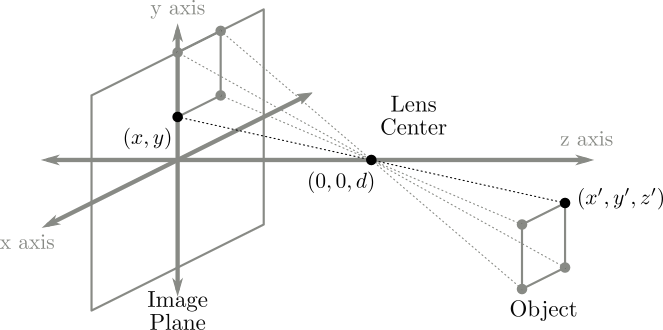
\includegraphics[width=0.75\textwidth]{figures/perspective.png}
  \caption{Perspective projection model.}
  \label{fig:perspective}
\end{figure}

In the context of image registration, we would like to know how changes in the relative position and orientation between the camera and observed scene affect projected coordinates.  However, it is not possible to express the coordinate transform between $i_1$ and $i_2$ as a function of $\bm{x}$, as the transform depends on the physical location of features in 3D space which is generally unknown.  However, assumptions can sometimes be made which simplify the transform significantly.

In many remote sensing applications, the distance to the scene is much larger than the distance to the lens center ($z' \gg d$) and the spacecraft's field of view is narrow.  In this setting, it is possible to show that small changes in attitude manifest as apparent translational motion of the scene.

%% FIXME - Proof

%% WIP Proof

%% With this result, the coordinate transform has now been simplified to

In other words

$$f(\bm{x}) = R_{\theta} \left(\bm{x} - [d \tan(\alpha),\, d \tan(\phi)]^T \right)$$
where $\theta$, $\phi$ and $\alpha$ are the spacecraft roll, pitch and azimuth.

This reduces the registration problem in many space science applications from a coordinate transform model of perspective projection, to a simple rigid model with translation and rotation in the image plane.


\begin{figure}
  \centering
  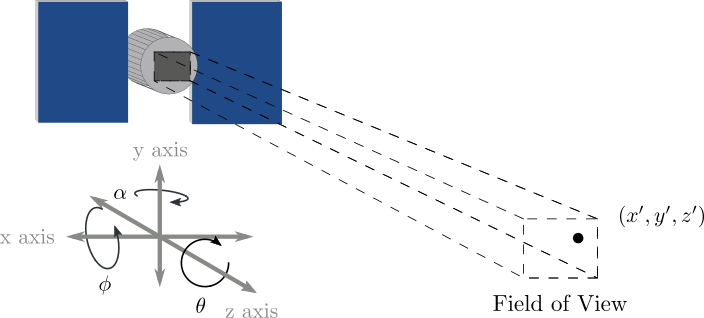
\includegraphics[width=0.75\textwidth]{figures/perspective_approx.png}
  \caption{Distance field of view of spacecraft, along with 6 degrees of freedom.}
\end{figure}

\subsection{Elastic}

When the type of transform is unknown or more complicated, elastic transforms can be used to correct for misalignment.  This can arise in situations where a 3D scene is projected through an optical system onto a 2D plane, but unlike perspective projection, there are large depth variations which occlude parts of the scene.  Objects which appear in one image may be completely obscured in the other, which is increasingly difficult to account for as the number of occlusions increases.  In these settings, a more general coordinate transform which can map more arbitrary distortions is preferred.

Elastic methods can either operate over the image as a whole (global), or apply different transforms to regions of the image separately (local).  An example of a global elastic method is the \emph{bivariate polynomial} transform, in which the x and y coordinates are fed through a pair of polynomial functions.

$$u = \sum_{l=0}^m \sum_{j=0}^i a_{ij} x^l y^{j - l}$$

$$v = \sum_{l=0}^m \sum_{j=0}^i b_{ij} x^l y^{j - l}$$
where $[x,\,y]$ are the original coordinates, $[u,\,v]$ the transformed coordinates, and $a_{ij}$ and $b_{ij}$ are constant parameters controlling the transform.

Local methods are more general than global methods and can handle distortions that global methods cannot, such as deformable objects, complex 3D surfaces, and object motion within the scene.  While these methods are more powerful, there is a tradeoff with computational complexity as the number of parameters increases.  An example of a local elastic coordinate transform is piecewise spline interpolation.

Figure \ref{fig:classes} is a diagram which illustrates examples of some of these transform classes.

\begin{figure}
  \centering
  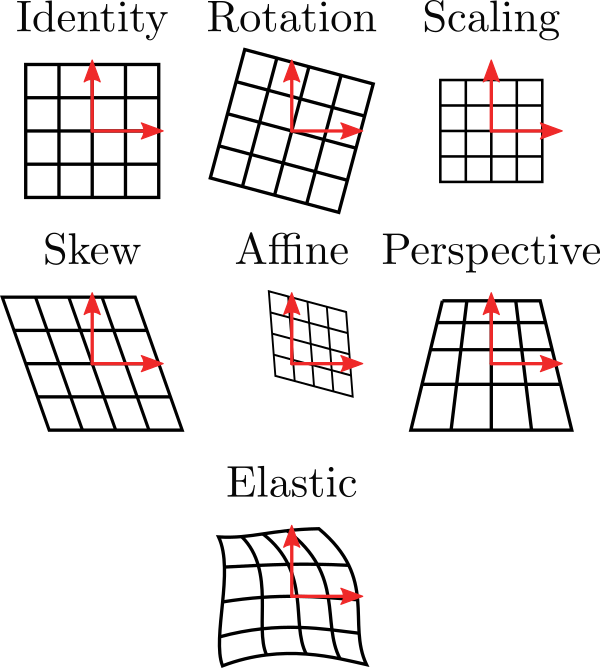
\includegraphics[width=0.5\textwidth]{figures/transforms.png}
  \caption{Visualizations of several coordinate transformations of a grid with origin prior to transformation shown with red arrows.}
  \label{fig:classes}
\end{figure}

\section{VISORS Mission}

The VIrtual Super-resolution Optics with Reconfigurable Swarms (VISORS) mission, due to be launched by NASA in 2023, is a heliophysics CubeSat mission designed to study the Sun's atmosphere (corona) at a finer scale than has been achieved in previous missions.  Its primary mission is to reveal the heating process which causes the corona to be over 1000 times hotter than its surface (photosphere), which has been a central problem in heliophysics for decades.

Observations made in x-ray and extreme ultraviolet (EUV) have provided hints on this heating process, but the structure and precise mechanism of the heating have yet to be observed directly.  A leading hypothesis is that the heating is constrained to narrow sheets which transfer energy from the Sun's surface into the corona.  The expected scale of these sheets is on the order of 100km \cite{klimchuk2015}, or about 150 milli-arcseconds (mas) when viewed from Earth's orbit, but no existing coronal imagers have been able to reach this resolution.

VISORS consists of two 3U spacecraft known as the optics spacecraft (OSC) and detector spacecraft (DSC), which carry instrumentation for taking measurements in extreme ultraviolet (EUV) range.  These two spacecraft will fly in formation 40 meters apart aligned along an axis pointed at the region of interest on the Sun during science mode.  The OSC focuses incoming light using a novel diffractive element known as a photon sieve while simultaneously using its solar panels to block off-axis light from entering the DSC.  The DSC will be positioned on the focal plane corresponding to He II emission line at 30.4 nm.  In particular, the OSC uses a diffractive optical element known as a photon sieve, which can outperform equivalent reflective optics due to tighter manufacturing tolerances \cite{oktem}.

%% FIXME - wavelength mentioned before this point

VISORS is what is known as a \emph{virtual} telescope.  In contrast to other non-virtual space telescopes such as Hubble (visible light) and the Solar Dynamic Observatory (EUV), the focusing optics and detector fly on separate spacecraft which allows the design to support large focal lengths without significantly increasing spacecraft volume and to reconfigure the focused wavelength after launch by adjusting spacecraft separation.

In addition to its contributions to heliophysics, VISORS will serve as a technology demonstration of diffractive, distributed telescopy and precision satellite formation flying.

%% FIXME - move sun further away from optics spacecraft

\begin{figure}
  \centering
  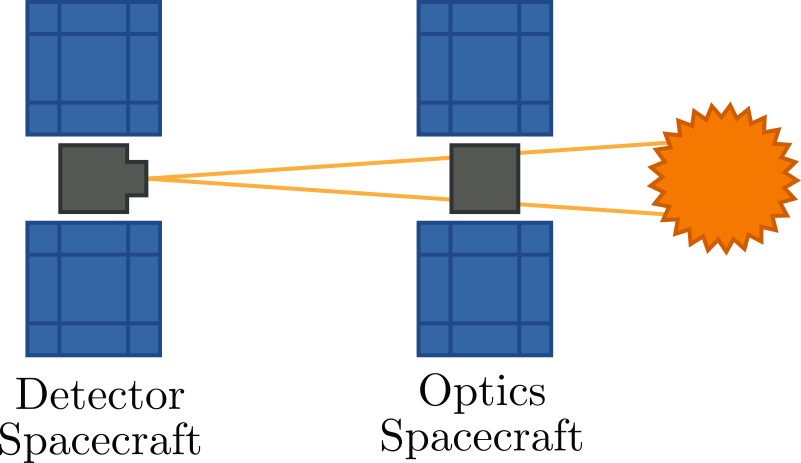
\includegraphics[width=0.5\textwidth]{figures/satellite.png}
  \caption{Pictoral representation of VISORS in formation flying configuration.}
\end{figure}

\section{Thesis Outline}

Chapter \ref{chap:preliminaries} introduces classes of image registration and describes popular registration methods from each class, and details the method of subpixel registration.
Chapter \ref{chap:multiframe} introduces the idea of multiframe registration and relates it mathematically to the two-frame problem.  I introduce a new multiframe registration method and explain how it is approximately optimal in an ML sense.
Chapter \ref{chap:experiments} contains numerical registration experiments under various settings, a description of the pipeline used to generate the test images, and some tests involving other classes of images unrelated to the VISORS project.

\chapter{Preliminaries} \label{chap:preliminaries}

\section{Review of Global Registration Methods} \label{sec:methods}

Most registration algorithms can be assigned to two broad categories known as area-based and feature-based methods.  These registration classes vary primarily in the steps leading up to transform estimation, while the image transformation step is generally unchanged for a given motion model.  In feature-based methods, localized structures such as lines, regions or points, known as \emph{features}, are detected and corresponded in the reference and sensed images during the feature detection and feature estimation steps.  In area-based methods, these steps are omitted entirely 

In this section, I focus primarily on the first three steps before performing the coordinate transform, namely feature detection, feature matching, and transform model estimation.

\subsection{Correlation Based Methods}
\subsubsection{Cross-Correlation}

The most straightforward of all methods, direct correlation, is conceptually simple and works for many classes of transforms.

%% FIXME - why is normalization so crucial

Note that the normalization here is crucial so that the intensities of $i_1$ and $i_2$ do not influence the maximum.  We call this measure normalized cross-correlation (NCC) \cite{brown}.

%% only works when $f$ is a simple linear translation, $f(\bm{x}) = \bm{x} - \bm{c}^*$.

$$
\begin{aligned}
\hat{f} &= \arg \max_{f \in F} \text{NCC}(i_1, f(i_2)) \\
&= \arg \max_{f \in F} \frac{\sum_{\bm{x} \in X} i_1(\bm{x})i_2(f(\bm{x}))}{\sqrt{\sum_{\bm{x} \in X} i_1(\bm{x})^2}}
\end{aligned}
$$
where $F$ is some class of coordinate transforms.  $f(i_2)$ is shorthand for a transformed imaged such that $f(i_2)(\bm{x}) = i_2(f(\bm{x}))$.  Practically, the time required to search the space of all possible transforms for a given application makes this approach infeasible, so $F$ is often restricted to translations for this method.

$$
\hat{c} = \arg \max_{\bm{c}} \frac{\sum_{\bm{x} \in X} i_1(\bm{x})i_2(\bm{x} - \bm{c})}{\sqrt{\sum_{\bm{x} \in X} i_1(\bm{x})^2}}
$$


%% $$ f^* = \arg \max_{\hat{f}} \sum_x i_1(x)i_2(\hat{f}(x)) = \arg \min_{\hat{f}} \sum_x e(x)^2 $$

Related similarity measures which are sometimes used in place of normalized cross-correlation are sum of squared error (SSE)

$$
\text{SSE}(i_1, f(i_2)) = \sum_{\bm{x} \in X} (i_1(\bm{x}) - i_2(f(\bm{x})))^2
$$

and correlation coefficient

$$
\text{Corr}(i_1, f(i_2)) = \frac{\text{cov}(i_1, f(i_2))}{\sigma_1 \sigma_2} = \frac{\sum_{\bm{x} \in X} (i_1(\bm{x}) - \mu_1)(i_2(f(\bm{x})) - \mu_2)}{\sqrt{\sum_{\bm{x} \in X} (i_1(\bm{x}) - \mu_1)^2 \sum_{\bm{x} \in X}(i_2(f(\bm{x})) - \mu_2)^2}}
$$
where $\mu_1$, $\mu_2$, $\sigma_1$, $\sigma_2$ are the means and variances of $i_1$ and $i_2$ over $X$.

While cross-correlation methods are very old, they continue to see widespread use because of ease of implementation in hardware (NCC can be efficiently implemented using multiply-accumulate hardware) and because limiting $f$ to translations isn't significantly restrictive for many scenarios.

In practice though, cross-correlation still succeeds on natural images in the presence of slight rotational, scalar or even non-linear distortions.

\subsubsection{Selective Similarity Detection Algorithm}

In standard correlation methods, the sum over $X$ for each candidate $f$ must be computed in full before a maximum is found.  Barnea, Silverman \cite{barnea} propose a class of alternative algorithms which greatly improve computation time in two ways.  The paper calls these algorithms selective similarity detection algorithms (SSDAs), of which one is presented here.

First, the paper uses absolute sum of errors (ASE) as a similarity measure, which requires no costly multiplications unlike NCC or SSE.

$$
ASE(i_1, f(i_2)) = \sum_{\bm{x} \in X} |i_1(\bm{x}) - i_2(\bm{x} - \bm{c})|
$$

The second optimization uses early stopping and requires that the sum over $X$ be implemented sequentially (e.g. as an iterative software loop).  For a particular candidate $\bm{c}$, the current value of the sum is compared to a threshold parameter $L$ after each iteration.  If the ASE surpasses this threshold, the number of iterations is recorded and the algorithm moves on to the next candidate.  If an candidate computation never exceeds $L$, then the final ASE is recorded instead.

Finally, the candidate with the lowest ASE is selected.  If all candidates surpassed the threshold, then the candidate with the most number of iterations before passing the threshold is selected.

\begin{figure}
  \centering
  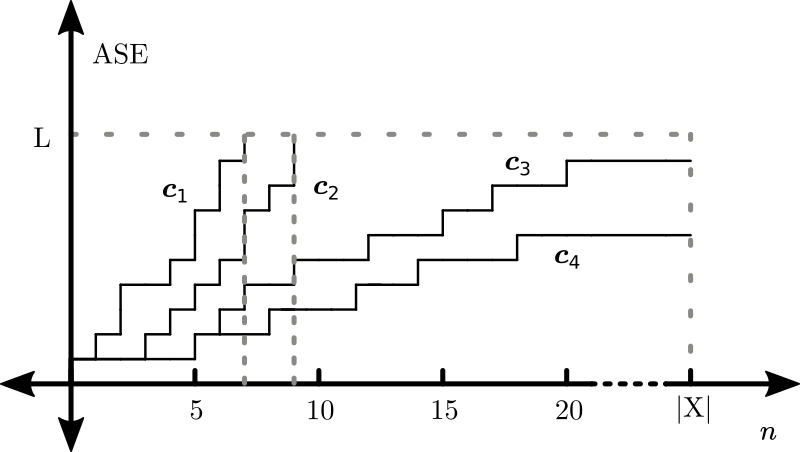
\includegraphics[width=0.75\textwidth]{figures/ssda.png}
  \caption{
    Error accumulation curves for candidates $\bm{c}_1$, $\bm{c}_2$, $\bm{c}_3$ and $\bm{c}_4$.  Error computation for $\bm{c}_1$ and $\bm{c}_2$ terminated early at 7 and 9 iterations.  $\bm{c}_4$ is the best estimate for offset, followed by $\bm{c}_3$, $\bm{c}_2$ and $\bm{c}_1$.
  }
\end{figure}

SSDA requires selection of parameter $L$.  A choice of $L$ too high limits efficiency gains while a choice of $L$ too low can lead to suboptimal results.  However, this algorithm offers potentially orders of magnitude in speed improvements over correlation methods which makes it appropriate for time-sensitive or computationally under-powered applications.

\subsection{Feature Based Methods}

Feature-based methods involve a preprocessing step known as \emph{feature detection}, where notable structures in both images are located.  These structures can come in a variety of forms and can correspond to different kinds of objects depending on the context.  For example, images being registered in a remote sensing context could contain features such as amorphous regions (forests, lakes, fields), line segments (roads, buildings), or single points (street intersections, region corners).  There are many algorithms capable of extracting these features and the optimal choice of algorithm is highly dependent on the target scene.  In general, a desirable property of these algorithms is that the same features can be detected in both images and that these features are robust against corruption introduced by intensity mapping function $g$ or noise \cite{zitova}.  In particular, the SIFT \cite{sift} and MSER \cite{mers} algorithms have gained widespread popularity in computer science as feature detection algorithms.

Some features in the sensed image may not have a matching counterpart in the reference image due to occlusions or because their counterpart is outside of the field of view. A desirable property of the feature matching algorithm is that incorrect matches are eliminated or assigned a low score so that parameter estimates in the later transform estimation step are not skewed \cite{zitova}.

\subsubsection{RANSAC}

%% section 5.1.4 \cite{french}

RANSAC, or RAndom SAmple Consensus, is an iterative parameter estimation method which is robust to outliers \cite{french}.  In the context of image registration, RANSAC is sometimes used to estimate the parameters of a perspective transform, where the outliers are erroneously matched pairs of features.

RANSAC begins by selecting a random subset of matched feature pairs and computing a hypothetical set of transform parameters.  In the case of perspective projection, this is simply solving a linear system.  The quality of this estimated coordinate transform is evaluated by transforming the coordinates of all features in the reference image and aggregating the error for all pairs.  This estimated transform is then stored along with its aggregate error, and the process is repeated for a new randomly selected subset of feature pairs until a predetermined number of transforms has been estimated.  The transform with the smallest aggregate error is then chosen as the algorithm's result.

RANSAC is unique among the methods described in this chapter in that it is non-deterministic and repeated trials on the same dataset can yield different results.  Additionally, while RANSAC is robust to outliers, it is not especially immune to measurement noise which causes the number of incorrectly paired features to rise \cite{french}.

%% \subsection{Optimization Based Methods}

\subsection{Information Based Methods}

Viola and Wells \cite{viola} introduced a new class of registration methods in 1994 based on entropy or information content of image pairs.  This class of methods has proven effective in multimodal registration so it has achieved significant popularity in medical imaging.

The number of unique messages that can be encoded given a message length of $n$ and $s$ unique symbols is $s^n$.  However, a desirable property of information is that information should grow linearly with message length.  A message which is twice as long should contain twice as much information.  Therefore, in the context of information theory, information is defined as

$$
H = \log s^n = n \log s
$$

From the first formulation, it is apparent that information grows linearly with $n$.  Another interesting feature of this measure is that if there is only one symbol, we know exactly what the message will be and so it contains no information $(H = n \log 1 = 0)$.  This suggests that entropy can also be viewed as a measure of uncertainty.

A disadvantage of this definition of entropy is that it assumes all symbols are equally likely to occur in a message, which is generally not true in physical systems.

An alternative measure of information takes this into account by weighting the entropy by the probability that symbols occur.  This is known as Shannon entropy.  For a set of $s$ symbols with probabilities $p_1, ..., p_s$ of occuring, Shannon entropy is given as

$$
H = \sum_k p_k \log \frac{1}{p_k} = - \sum_i p_k \log p_k
$$

Like the unweighted entropy measure, Shannon entropy can be viewed as a measure of uncertainty.  If a particular symbol has a very high probability of occuring, our uncertainty about the message decreases and hence information decreases.  If all symbols have an equal probability of occuring, entropy is maximized.  Thus Shannon entropy may also be considered as a measure of spread of a probability distribution \cite{hartley}.  A distribution with most mass concentrated around a few peaks will have low entropy while a more uniform distribution will have higher entropy.

To compute Shannon entropy of an image, all possible intensity values of the pixels can be interpreted as symbols in the message.  For an image with bit depth of 8 bits, one can collect all the intensity values into a histogram in order to compute $p_0, ..., p_{255}$, as shown in Figure \ref{fig:histogram}.

\begin{figure}
  \centering
  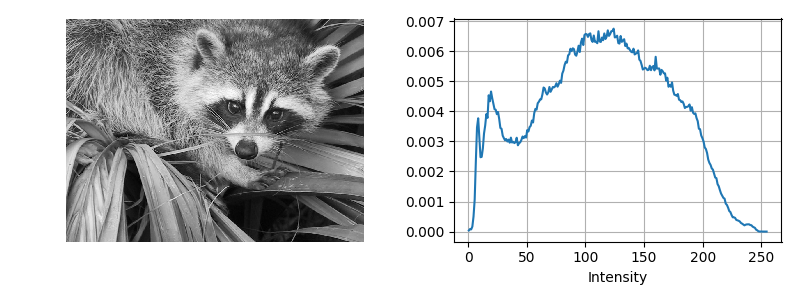
\includegraphics[width=1\textwidth]{figures/histogram.png}
  \caption{
    An image and its intensity histogram
  }
  \label{fig:histogram}
\end{figure}

Now that we can compute entropy for images we must introduce one more concept before registration can occur, joint histograms.  A joint histogram is a 2D function which, for all possible pairs of intensities, describes how many times intensity pairs occur for a pair of registered images.  For example, if a joint histogram has value 17 at coordinate [33, 34], then for this particular registration there are 17 pixels in which the first image has intensity 33 and the second has intensity 34.  In the case of two 8 bit images, the joint histogram is a 256x256 image.  An example joint histogram for two images is shown in Figure \ref{fig:joint_histogram}.

\begin{figure}
  \centering
  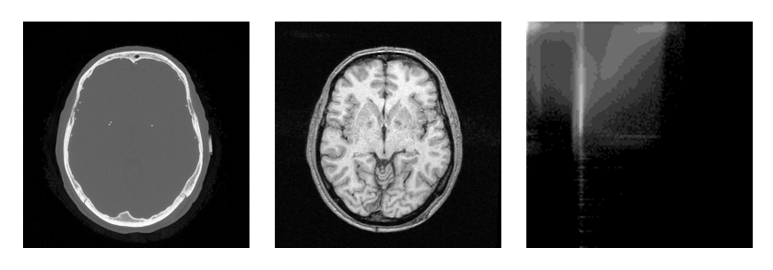
\includegraphics[width=1\textwidth]{figures/feature_space.png}
  \caption{
    Two registered images and their joint histogram, or feature space.
  }
  \label{fig:joint_histogram}
\end{figure}

The joint histogram changes with the alignment of the images.  For a correctly aligned pair of images, structures within the image align and vary with each other, so we expect the intensities to correlate which manifests as clustering in the joint histogram.  As the image pair becomes misaligned, more greyscale combinations are introduced and the joint histogram exhibits more uniformity.  By measuring this uniformity we now have a similarity measure for registration.

Formally, the joint Shannon entropy for a pair of registered images

$$
H(i_1, f(i_2)) = -\sum_{m, n} p(m, n) \log p(m, n)
$$
where $p(i, j)$ is the joint histogram of $i_1$ and candidate registered $f(i_2)$ in the region of overlap $X$.
%% <!-- FIXME -->

However, a problem that can occur when joint entropy is used directly is that low entropy (high degree of reported alignment) can occur for invalid registrations if the images contain large regions of uniform intensity.  For example, if the images in the figure above are aligned so that only their corners containing background overlap, the joint histogram will have approximately a single peak and the joint entropy will be very low.  To account for this, one can make use of the marginal entropies to penalize alignments where the region $X$ contains little information in the images.  This is known as mutual information.

$$
MI(i_1, f(i_2)) = H(i_1) + H(f(i_2)) - H(i_1, f(i_2))
$$

With this new measure, if the overlap region contains little information, terms $H(i_1)$ and $H(f(i_2))$ will be small and counteract joint entropy.  Also note that since mutual information contains $-H(i_1, f(i_2))$, minimizing joint entropy is related to maximizing mutual information.

The abiliity of mutual information based methods to handle images with differing distributions of pixel intensities makes it uniquely suited for multimodal image registration applications.  Especially in medical applications, mutual information based registration can be used to register images of the same organ made by different instruments (e.g. PET and CT).

\subsection{Frequency Based Methods}

If an acceleration over correlation-based methods is needed or the images were acquired under frequency dependent noise, Fourier methods are often preferred.  These methods exploit the Fourier representation of images in the frequency domain and have shown better robustness against illumination differences between $i_1$ and $i_2$.

\subsubsection{Phase Correlation}

Phase correlation was originally proposed for registering linearly translated images.  It takes advantage of the Fourier Shift theorem, which states that translating an image and taking its Fourier transform is equivalent to multiplying the Fourier transform of the original untranslated image by a complex exponential.

Computing the cross-power spectral density (CPSD) we can directly obtain this complex exponential.

$$
i_2(\bm{x}) = i_1(\bm{x} - \bm{c}^*)
$$

$$
CPSD(i_1, i_2)(\bm{\omega}) = \frac{\tilde{i}_1(\bm{\omega}) \overline{\tilde{i}_2(\bm{\omega})}}{|\tilde{i}_1(\bm{\omega}) \overline{\tilde{i}_2(\bm{\omega})}|} =
\frac{\tilde{i}_1(\bm{\omega}) \overline{\tilde{i}_1(\bm{\omega}) e^{-j \langle \bm{\omega}, \bm{c}^* \rangle}}}{|\tilde{i}_1(\bm{\omega}) \overline{\tilde{i}_1(\bm{\omega}) e^{-j \langle \bm{\omega}, \bm{c}^* \rangle}}|} = e^{j \langle \bm{\omega},  \bm{c}^* \rangle}
$$
where $\tilde{i}_1$ and $\tilde{i}_2$ are the Fourier transforms of $i_1$ and $i_2$.  The final estimate for $\bm{c}_0$ is obtained by a final inverse Fourier transform of the CPSD, yielding a delta at location $\bm{c}_0$.

\begin{gather*}
  PC(i_1, i_2)(\bm{x}) = \mathcal{F}^{-1}\left[ CPSD(i_1, i_2) \right](\bm{x}) = \delta(\bm{x} - \bm{c}^*) \\
  \hat{c} = \arg \max_{\bm{x}} PC(i_1, i_2)(\bm{x})
\end{gather*}

An important consideration here is that the Fourier Shift theorem only holds when translation is circular.  In practice, the phase correlation method still works if the region of overlap is sufficiently large.  Foroosh, Zerubia, Berthod \cite{foroosh} propose a prefilter which can be applied to both images before phase correlation to reduce these effects.

\section{Subpixel Registration} \label{sec:subpixel}

We will now turn our attention to a special class of translational registration methods known as \emph{subpixel} methods.  Unlike non-subpixel translation methods which return a vector of integers representing the coordinate shift between images in each axis, subpixel methods assume the scene being observed exists at a higher resolution than the observations and seek to find a fractional value for this shift.  In real imaging systems, the resolution ratio between the scene and observations is usually infinite as the scene is a continuous function.  However, in practice this ratio is often assumed to be finite and the scene assumed to exist on a discrete high resolution grid which captures the features of the scene being studied in sufficient detail.

This requires us to adjust the image registration model given in the introduction to include some notion of downsampling.  First we define a pair of high resolution images $h_1$ and $h_2$ which live on a high resolution grid.  The observed images $i_1$ and $i_2$ are downsampled versions of these high resolutions images corresponding to the same field of view.  The downsample factor between the high resolution grid and low resolution grid is denoted by positive integer $d$.

\begin{eqnarray*}
  i_2[\bm{x}] = h_{2}[d \bm{x}] \\
  i_1[\bm{x}] = h_{1}[d \bm{x}] \\
  \bm{x} \in X
\end{eqnarray*}

Now instead of aligning $i_1$ and $i_2$ like non-subpixel methods, subpixel registration seeks to align the high resolution images without directly observing them:

$$
h_{2}[\bm{x}_h] = h_{1}[\bm{x}_h - \bm{c}] \,\, \forall \bm{x}_h \in X_h
$$
where $\bm{x}_h \in X_h$ is a high resolution coordinate of the high resolution set of points $X_h$.

In this section, I introduce 2 subpixel registration methods and highlight advantages and disadvantages of each.

\subsection{Interpolation and Registration}

A straightforward way to achieve subpixel registration is to make use of interpolation techniques to boost the accuracy of the misalignment estimate.

Some methods involve interpolating the observed images before applying a standard non-subpixel registration technique such as cross-correlation to the upsampled images \cite{interp}.

Other methods make use of the correlation surface obtained from the low resolution images, then upsample or fit a continuous function to the surface before searching for a maximum. Many types of interpolation have been employed, such as nearest neighbor, bilinear, spline and sinc interpolation \cite{interp2}.  A classic technique involves zero-padding the correlation result from one of the Fourier-based methods described previously before inversion, which effectively applies sinc interpolation while benefitting from the efficiency of FFT algorithms.

$$\hat{\bm{c}} = \arg \max_{\bm{x}_h \in X_h} \text{IFFT}\left( \text{Zeropad}_d \left( \text{FFT}(i_1) \cdot \overline{\text{FFT}(i_2)}\right)\right)[\bm{x}_h]$$

However, a major downside to these subpixel methods is that computational cost often scales rapidly with image size and downsample factor $d$.  For example, using the zero-padded IFFT technique on a square image 1024 pixels wide requires computation and storage of an IFFT of size 102400 on either side, not feasible on modern workstations \cite{guizar}.

\subsection{Accelerated Interpolation via IDFT}

To get around the computational challenges associated with the zero-padded IFFT method, Guizar-Sicairos et al. \cite{guizar} developed a mathematically equivalent algorithm which is faster and much more resource efficient.  It uses a two step coarse-to-fine approach to first find the approximate peak location on the original low-resolution grid, then applies an upsampled IDFT to a region of pixels around this peak to obtain a fine registration estimate.

$$\hat{\bm{c}}_{\text{coarse}} = \arg \max_{\bm{x} \in X} \text{IFFT} \left( \text{FFT}\left(i_1\right) \cdot \overline{\text{FFT}\left(i_2\right)} \right)[\bm{x}]$$

$$\hat{\bm{c}} = \arg \max_{\bm{x}_h \in \text{N}(\hat{\bm{c}}_{\text{coarse}})} \text{UpsampIDFT} \left( \text{FFT}\left(i_1\right) \cdot \overline{\text{FFT}\left(i_2\right)} \right)[\bm{x}_h]$$
where $N(\hat{\bm{c}}_{\text{coarse}})$ is a neighborhood of pixels around $\hat{\bm{c}}_{\text{coarse}}$ and  $\text{UpsampIDFT}$ is an inverse DFT operation with an output size larger than its input size.

This two step process is illustrated in Figure \ref{fig:guizar}.

\begin{figure}
    \centering
    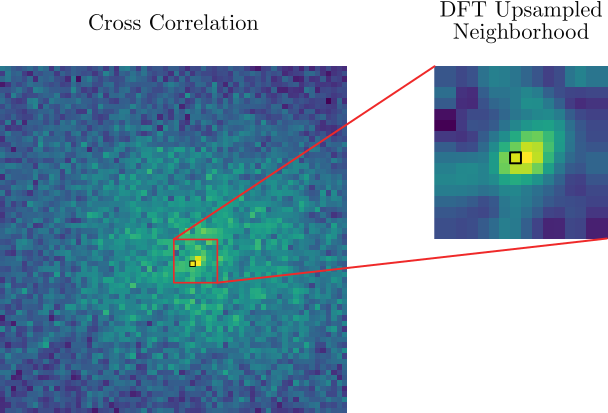
\includegraphics[width=0.5\textwidth]{figures/guizar_upsample.png}
    \caption{Two steps of Guizar-Sicairos's method.  A coarse peak location is found in the original correlation surface, then a small neighborhood around this peak is upsampled via IDFT to get the fine estimate.}
    \label{fig:guizar}
\end{figure}

\chapter{Multiframe Registration} \label{chap:multiframe}

Multiframe registration is a generalization of image registration from a pair of images to a set of images.  This image set may be ordered, as in the case of a sequence of frames, or unordered.  The idea remains the same as classical registration in that the goal is to align template images in the sequence with a reference image.

There are many applications of multiframe registration, such as chromatic aberration correction \cite{aberration}, motion stabilization in video \cite{smoothing}, super resolution \cite{farsiu2004}, noise reduction and image compositing \cite{salient}.

In this chapter, I introduce a mathematical model for the problem of multiframe registration, describe a multiframe registration algorithm developed for the constant translational motion model in the the VISORS project, then show how this method is derived from the maximum likelihood solution to multiframe registration.

\section{Multiframe Registration Problem Model} \label{sec:model}

Let $i_j$ and $i_k$ be two images from a set of K images.  In the classical registration problem, we would like to relate these two images such that 

$$
i_k[\bm{x}] = i_j[f_{j,k}(\bm{x})] \,\, \forall \bm{x} \in X
$$

by finding the coordinate transform $f_{j,k}$ from the jth frame to the kth frame.  In the multiframe setting, not only do we wish to find $f_{j,k}$, but also some or all of the $K(K - 1)$ coordinate transforms which relate any two images in the set.

Multiframe registration methods take varying approaches when choosing template and reference images.  Methods taking the \emph{anchoring} approach choose a single anchor frame from the set of images and register all other images against this frame.  These methods are sometimes used when motion between frames is random, such as the case of random vibrations affecting a camera system.

An alternative is the \emph{progressive} approach, where pairs of adjacent frames in an ordered image sequence are taken to be the reference and sensed images.  This is often used in situations where there is some prior knowledge on the motion between adjacent image pairs.  For example, in a handheld camera one would expect motion between adjacent frames to change slowly over time, as the movements induced by hand tremors are relative slow compared to the shutter frame rate \cite{smoothing}.

In both cases, it is usually desirable that the found coordinate transforms exhibit properties of consistency known as the \emph{Jacobi Identity} and \emph{Skew Anti-Symmetry} properties \cite{farsiu2005}.

The Jacobi Identity property states that the application of the coordinate transform from frame $j$ to frame $k$, then the transform from k to l should be the same as the transform from j to l.

\begin{equation}
  f_{j,k}(f_{k,l}(\bm{x})) = f_{j,l}(\bm{x})
  \label{eqn:jacobi}
\end{equation}

for $j,k,l \in 1, ..., K$.

In a similar vein, the skew anti-symmetry property states that applying coordinate transform $f_{k,j}$ immediately after $f_{j,k}$ should yield the original coordinate.

\begin{equation}
  f_{k,j}(f_{j,k}(\bm{x})) = \bm{x}
  \label{eqn:antiskew}
\end{equation}

for $j,k \in 1, ..., K$.

These properties (illustrated in Figure \ref{fig:properties}) serve to constrain the set of found coordinate transforms to a solution which is physically realizable \cite{milanfar}.

We may impose additional constraints on the coordinate transform solution set if there is extra prior knowledge about the class of transforms.  In the VISORS project, we assume that motion is purely translational and constant between frames. i.e.

\begin{eqnarray}
  f_{j,k}(\bm{x}) = \bm{x} - \bm{c}(k - j) \\
  f_{j,k}(\bm{x}) = f_{l,m}(\bm{x})
  \label{eqn:constant}
\end{eqnarray}

for $j,k,l,m \in 1, ..., K$ when $k - j = m - l$.  $\bm{c}$ is the interframe drift vector in pixels.

Plugging these constraints into the left-hand side of Equations \ref{eqn:jacobi} and \ref{eqn:antiskew}, it is easy to see the Jacobi and skew anti-symmetry properties are satisfied.

\begin{figure}
  \centering
  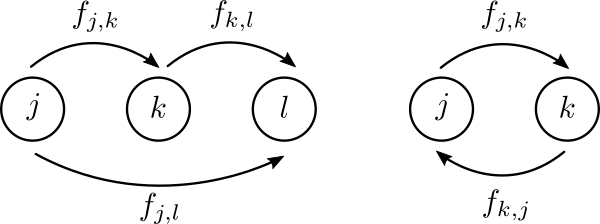
\includegraphics[width=0.6\textwidth]{figures/properties.png}
  \caption{Jacobi Identity and Skew Anti-Symmetry properties.}
  \label{fig:properties}
\end{figure}

%% \section{Multiframe Registration with All Frames}

%% The algorithm presented by Guizar-Sicairos, Thurman, Fienup is a 2-step subpixel registration method which first obtains a coarse, whole-pixel drift vector estimate from standard cross-correlation and then refines it by upsampling the cross-correlation with sinc interpolation.

%% The major argument of this paper is that the refined estimation step can be greatly accelerated by directly evaluating the DFT in a region around the coarse estimate as opposed to a zero-padded FFT technique.

%% A naive extension of this algorithm to a multiframe setting with constant translational motion constraint would be repeated application of the algorithm to adjacent frames in a progressive fashion, then an averaging of the estimated motion parameters to get a single estimate.

%% $$\hat{\bm{c}}_{\text{coarse}} = \text{mean}_{k=1}^{K-1} \left( \arg \max_{\bm{x} \in X} \text{IFFT} \left( \text{FFT}\left(i_k\right) \cdot \overline{\text{FFT}\left(i_{k+1}\right)} \right)[\bm{x}] \right)$$

%% $$\hat{\bm{c}} = \text{mean}_{k=1}^{K-1} \left( \arg \max_{\bm{x}_h \in \text{N}(\hat{\bm{c}}_{\text{coarse}})} \text{UpsampIDFT} \left( \text{FFT}\left(i_k\right) \cdot \overline{\text{FFT}\left(i_{k+1}\right)} \right)[\bm{x}_h] \right)$$

%% Since only two frames are correlated at a time and since the mean is sensitive to outliers, this method is not robust against noise and fails in low SNR settings, as will be shown in the numerical experiments section.

%% Instead, we can tweak this algorithm to jointly consider many frames in the sequence simultaneously before taking argmax to obtain an estimate.


%% First define \emph{correlation sum} (denoted $CS_1$ as the sum of all correlation surfaces between adjacent frames.  Due to the property described in  Equation \ref{eqn:constant} given in the previous section, the peak of the correlation surfaces all lie in the same location.

%% $$
%% CS_1 = \text{IFFT} \left(\text{FFT}(i_1) \cdot \overline{\text{FFT}(i_2)} + \text{FFT}(i_2) \cdot \overline{\text{FFT}(i_3)} + ... \right)
%% $$

%% Additionally, we need not only consider adjacent frames, but we can consider frames separated by 2 or more for better noise immunity.

%% $$
%% CS_k = \text{IFFT} \left(\text{FFT}(i_1) \cdot \overline{\text{FFT}(i_{1+k})} + \text{FFT}(i_2) \cdot \overline{\text{FFT}(i_{2+k})} + ... \right)
%% $$

%% Examples of correlation sums for experimental data are given in Figure \ref{fig:correlations}.

%% \begin{figure}
%%   \centering
%%   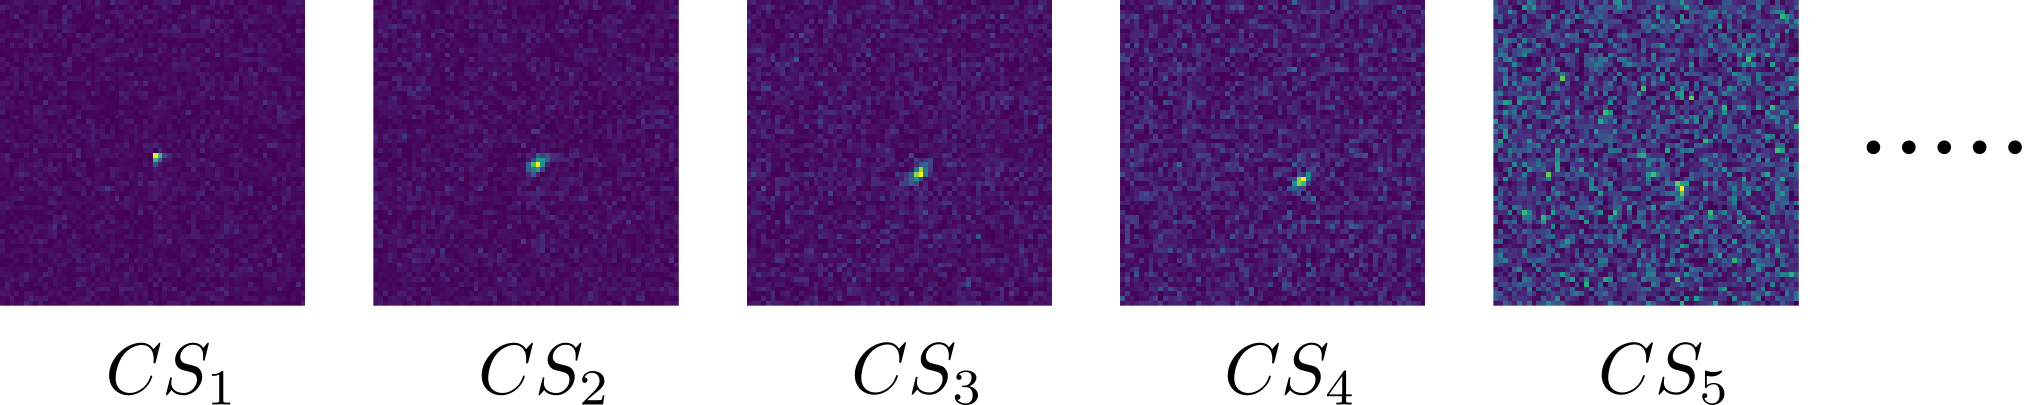
\includegraphics[width=0.75\textwidth]{figures/correlations.png}
%%   \caption{Sample correlation sum surfaces.}
%%   \label{fig:correlations}
%% \end{figure}

%% By substituting these correlation sums into Guizar-Sicairos's algorithm, we obtain a registration method which jointly considers all frames

%% $$
%% \hat{\bm{c}}_{\text{coarse}} = \text{mean}_{k=1}^{K-1} \left( \frac{\arg \max_{\bm{x} \in X} CS_k[\bm{x}]}{k} \right) \\
%% $$

%% $$
%% \hat{\bm{c}} = \text{mean}_{k=1}^{K-1} \left( \frac{\arg \max_{\bm{x}_h \in \text{N}(\hat{\bm{c}}_{\text{coarse}})} \text{UpsampIDFT} \left( \text{FFT}(CS_k) \right)[\bm{x}_h]}{k} \right)
%% $$

%% As we will see in the numerical experiments section, this algorithm yields significantly more accurate results than a direct application of the Guizar-Sicairos method due to stronger assumptions about interframe motion

\section{Multiframe Registration with All Frames} \label{sec:algorithm}

A naive extension of one of the algorithms described in section \ref{sec:methods} appropriate for constant translational motion might be repeated application of the algorithm to adjacent frames in a progressive fashion, then an averaging of the estimated motion parameters to get a single estimate.  For example, one might extend the algorithm given by Guizar-Sicairos for subpixel registration to multiple frames like so
$$\hat{\bm{c}} = \frac{\sum_{k=1}^{K-1} \text{Register}(i_k, i_{k+1})}{K-1}$$
where $\text{Register}(\cdot,\,\cdot)$ represents one of the algorithms given in section \ref{sec:methods}.

However, since only two frames are considered at a time, in low SNR settings $\text{Register}(\cdot,\,\cdot)$ may return an estimate which is wildly inaccurate.  As the mean is sensitive to outliers, this can seriously degrade the accuracy of the estimate.
Instead, one can use methods which jointly consider all adjacent image pairs to suppress noise before a motion estimate is made.

The method I propose in this section works by fusing correlation surfaces from many image pairs into a single surface before finding the maximum to make an estimate.  Not only does it use correlation surfaces from adjacent image pairs, but also all pairs separated by 2 or more frames for greater noise immunity.  One might believe that these higher order correlation surfaces contain redundant information which is already present in the surfaces for adjacent images, but the analysis in Section \ref{sec:optimality} suggests this is the right approach.

First define \emph{correlation sum} (denoted $CS_m$) as the sum of all phase correlation surfaces of image pairs separated by $m$.
$$CS_m[\bm{c}] = \sum_{k=1}^{K - m} (i_k \star_p i_{k+m})[\bm{c}]$$
where $\star_p$ is phase correlation.
Examples of correlation sums for experimental data are given in Figure \ref{fig:correlations}.

\begin{figure}
  \centering
  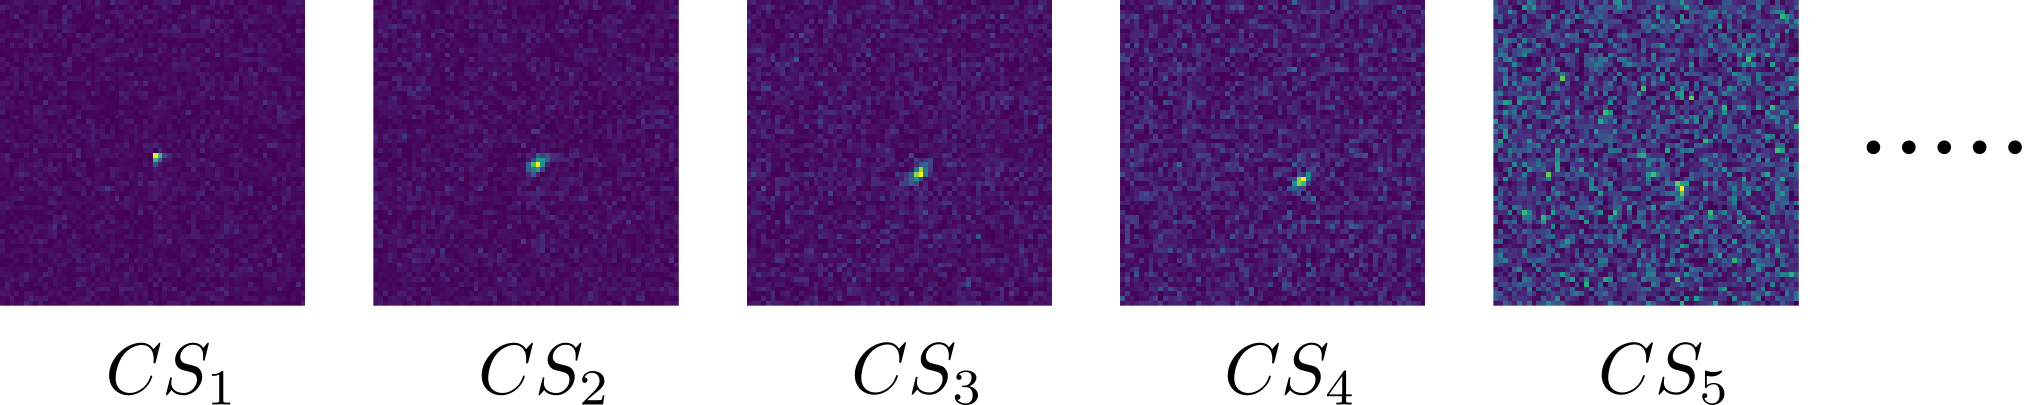
\includegraphics[width=0.75\textwidth]{figures/correlations.png}
  \caption{Sample correlation sum surfaces.}
  \label{fig:correlations}
\end{figure}

The location of the peak of the correlation sum varies with $\bm{c}m$, so in order to add all the correlation sums into a single surface, I scale them spatially so that their peaks coincide.  Finally, I add these scaled correlation sums, find the peak location.  This algorithm can be summarized mathematically as
\begin{align}
  \hat{\bm{c}} &= \frac{1}{K - 1} \arg \max_{\bm{c}} \sum_{m=1}^{K - 1} CS_m \left[\frac{m}{K - 1} \bm{c}\right] \\
  &= \frac{1}{K - 1} \arg \max_{\bm{c}} \blue{\sum_{m=1}^{K - 1}} \red{\sum_{k=1}^{K - m}} (i_k \star_p i_{k + m})\left[ \green{\frac{m}{K - 1}} \bm{c} \right]
  \label{eq:method}
\end{align}

The algorithm is illustrated in Figure \ref{fig:method} and has been color coded to correspond to Equation \ref{eq:method}.

\begin{figure}[h]
  \centering
  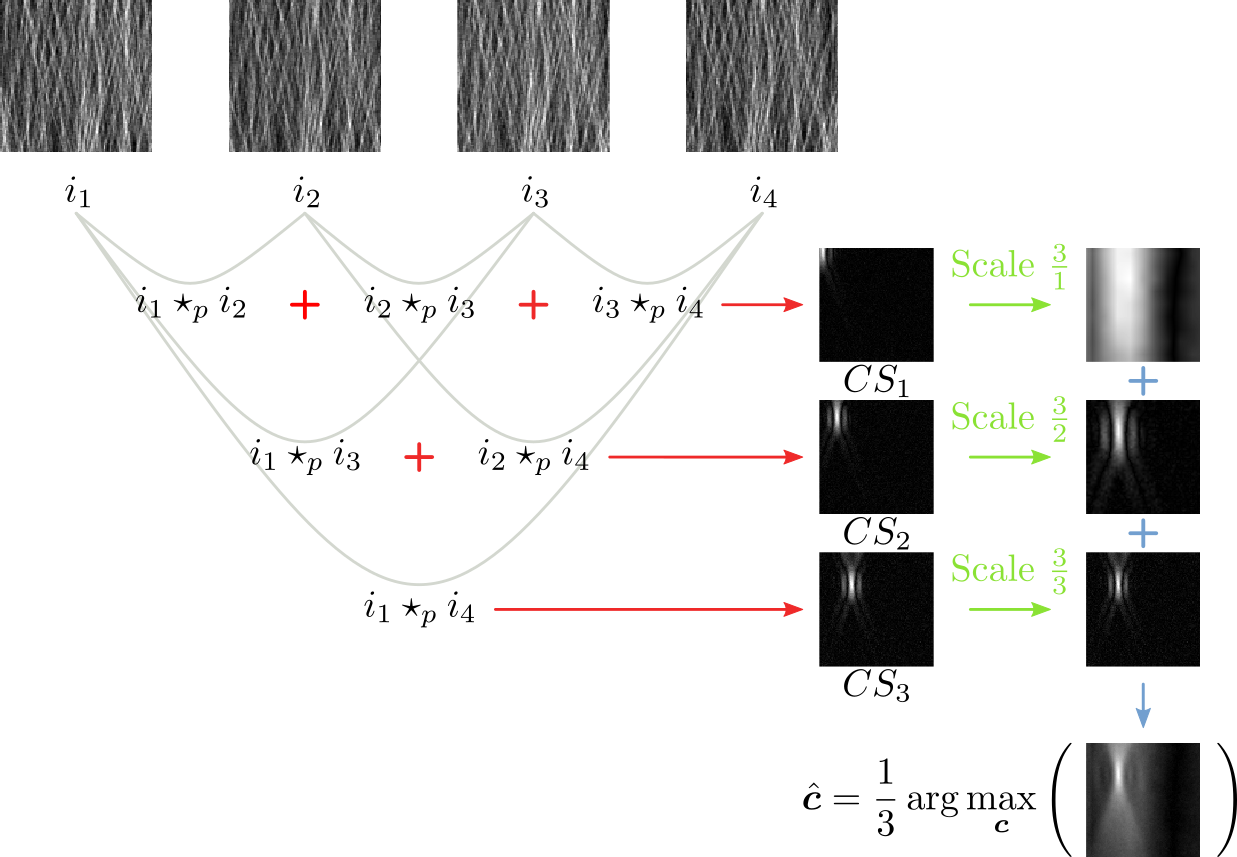
\includegraphics[width=0.9\textwidth]{figures/multiframe.png}
  \caption{Illustration of multiframe registration method.}
  \label{fig:method}
\end{figure}

As we will see in the numerical experiments section, this algorithm yields significantly more accurate results than a naively extended application of the Guizar-Sicairos method due to stronger assumptions about interframe motion.

\section{Optimality} \label{sec:optimality}

In this section, I show that the above algorithm is derived from the maximum-likelihood (ML) solution to the multiframe registration problem with a particular set of assumptions.  I first show the process of deriving the ML solution to a two frame registration problem, then use the same approach to extend to multiple frames and arrive at the final answer.

\subsection{Two Frames}

To derive the ML solution to the registration problem with two frames, I make the following simplifying assumptions

\begin{itemize}
  \item Images are circularly shifted rather than linearly shifted.
  \item Observations are corrupted with additive white Gaussian noise with variance $\sigma^2$.
\end{itemize}

Let $\mu = \left[ \mu_1, ..., \mu_N \right]^T$ be a vector representing the ground truth input scene.

Let $C_c(\cdot)$ be a circular shift operator by $c$ positions.

Let $i_1 = \left[i_{1,1}, ..., i_{1,N}\right]^T \sim \mathcal{N}(C_c(\mu), \sigma^2)$ be a noisy observation of $\mu$ shifted by integer $c$.

The likelihood of $i_1$ given $c$ is
$$P(i_1 | c) = \prod_{n=1}^N P(i_{1,n} | c) = \prod_{n=1}^N \phi \left( \frac{i_{1,n} - C_c(\mu)_n}{\sigma} \right)$$
where $\phi$ is the probability density function of the standard normal distribution.  Thus the ML solution for $c$ is

\begin{align*}
  \hat{c} &= \arg \max_c \ln P(Y | c) \\
  &= \arg \max_c \sum_{n=1}^N \ln \text{exp} \left[- \frac{(Y_n - C_c(\mu)_n)^2}{\sigma^2} \right] \\
  &= \arg \min \sum_{n=1}^N \left[Y_n - C_c(\mu)_n\right]^2 \\
  &= \arg \min_c \cancel{\sum_{n=1}^N Y_n^2} - 2\sum_{n=1}^N Y_n C_c(\mu)_n + \cancel{\sum_{n=1}^N \mu_n^2}
  && \eqcomment{Since the first and third terms are constant over $c$} \\
  &= \arg \max_c \sum_{n=1}^N Y_n C_c(\mu)_n
  = \arg \max_c \langle Y,\, C_c(\mu) \rangle
\end{align*}
where $\langle \cdot,\, \cdot \rangle$ is inner product.

Recognizing that the above inner product is a circular cross correlation, we conclude that argmax of cross correlation is the ML solution for two frames.

%% \cite{gcc}

$$\hat{c} = \arg \max_c \langle Y,\, C_c(\mu) \rangle = \arg \max_c (Y \star \mu)[c]$$
where $\star$ is circular cross correlation.

Note that the solution still depends on the ground truth $\mu$.  This will be addressed in the next section.

%% FIXME use M/m instead of K/k

\subsection{Multiple Frames}

Using the same approach as above I derive the maximum likelihood, but in a multiframe context.  The outline of this proof is as follows:

\begin{enumerate}
  \item Derive joint probability of observing all frames given the drift between frames.
  \item Derive ML solution to finding the drift assuming the ground truth scene is known.
  \item Since the ground truth is generally not known, substitute it with the average of the registered frames.
  \item Expand terms and recognize the expression is a sum of correlations between frames.
  \item Substitute sum of correlations with \emph{correlation sum} as defined in Section \ref{sec:algorithm}.
\end{enumerate}

Let $i_k = \left[i_{k,1}, ..., i_{k,N}\right]^T \sim \mathcal{N}(C_{ck}(\mu), \sigma^2)$ be the kth noisy observation of $\mu$ shifted by $ck$ in a sequence of $K$ frames of length $N$.  This is illustrated in Figure \ref{fig:multiframecirc}.

\begin{figure}
  \centering
  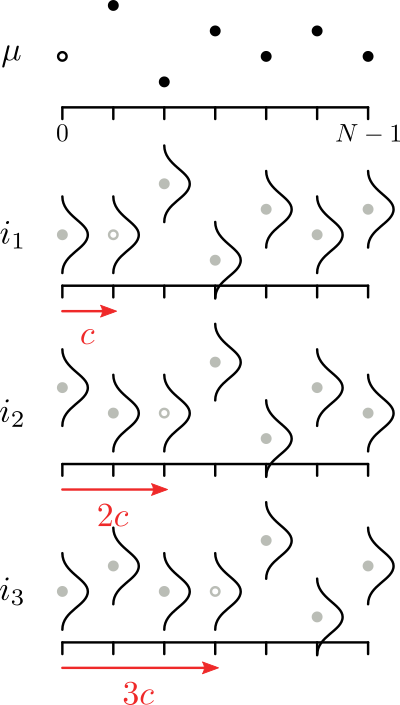
\includegraphics[width=0.45\textwidth]{figures/multiframecirc.png}
  \caption{Circularly shifted 1D observations corrupted with i.i.d. Gaussian noise.}
  \label{fig:multiframecirc}
\end{figure}

The likelihood of $i_1, ..., i_K$ is then

\begin{align*}
P(i_1, ..., i_K | c) &= \prod_{k=1}^K P(i_k | c) = \prod_{k=1}^K \prod_{n=1}^N P(i_{k,n} | c) \\
&= \prod_{k=1}^K \prod_{n=1}^N \phi \left(\frac{i_{k,n} - C_{ck}(\mu)_n}{\sigma} \right)
\end{align*}

And the ML solution for $c$ is

\begin{align*}
  \hat{c} &= \arg \max \ln P(i_1, ..., i_K | c) \\
  &= \arg \max_c \sum_{k=1}^K \sum_{n=1}^N \ln \text{exp} \left[- \frac{(i_{k,n} - C_{ck}(\mu)_n)^2}{\sigma^2} \right] \\
  &= \arg \min_c \sum_{k=1}^K \sum_{n=1}^N \left[ i_{k,n} - C_{ck}(\mu)_n \right]^2 \\
  &= \arg \min_c \sum_{k=1}^K \sum_{n=1}^N i_{k,n}^2 - 2i_{k,n}C_{ck}(\mu)_n + \mu_n^2 \\
  &= \arg \max_c \sum_{k=1}^K \sum_{n=1}^N i_{k,n}C_{ck}(\mu)_n 
  = \arg \max_c \sum_{k=1}^K \ip{i_k}{C_{ck}(\mu)}
\end{align*}

However, since the ground truth scene $\mu$ is generally not known in image registration problems, this solution is not directly usable.  Instead we can make an additional assumption that $\mu$ is equal to the average of the corrected frames.

$$\mu = \frac{C_{-c}(i_1) + ... + C_{-Kc}(i_K)}{K}$$.

Substituting this definition of $\mu$ into the above result yields

\begin{align*}
  \hat{c} &= \arg \max_c \sum_{k=1}^K \ip{i_k}{C_{ck}(\mu)} \\
  &= \arg \max_c \sum_{k=1}^K \ip{i_k}{C_{ck}\left(\frac{C_{-c}(i_1) +  ... + C_{-Kc}(i_K)}{K}\right)} \\
  & \eqlinecomment{Since $C$ is a linear operator and since $K$ does not depend on $c$:} \\
  &= \arg \max_c \sum_{k=1}^K \ip{i_k}{C_{ck}\left(C_{-c}(i_1)\right)} +  ... + \ip{i_{k,n}}{C_{ck}\left(C_{-Kc}(i_K)\right)} \\
  & \eqlinecomment{Since $C_a(C_b(\cdot)) = C_{a+b}(\cdot)$:} \\
  &= \arg \max_c \sum_{k=1}^K \ip{i_k}{C_{(k-1)c}(i_1)} +  ... +  \ip{i_k}{C_{(k-K)c}(i_K)} \\
  &= \arg \max_c \sum_{k=1}^K (i_k \star i_1) [(k - 1)c] + ... + (i_k \star i_K)[(k - K)c] \\
  & \eqlinecomment{Without loss of generality, assume the number of frames $K=4$:} \\
  & \begin{aligned}
    = \arg \max_c &\hphantom{{}+{}}
           (i_1 \star i_1)[0]  & {}+{} & (i_1 \star i_2)[-c] & {}+{} & (i_1 \star i_3)[-2c] & {}+{} & (i_1 \star i_4)[-3c] \\
    &{}+{} (i_2 \star i_1)[c]  & {}+{} & (i_2 \star i_2)[0]  & {}+{} & (i_2 \star i_3)[-1c] & {}+{} & (i_2 \star i_4)[-2c] \\
    &{}+{} (i_3 \star i_1)[2c] & {}+{} & (i_3 \star i_2)[c]  & {}+{} & (i_3 \star i_3)[0]   & {}+{} & (i_3 \star i_4)[-1c] \\
    &{}+{} (i_4 \star i_1)[3c] & {}+{} & (i_4 \star i_2)[2c] & {}+{} & (i_4 \star i_3)[c]   & {}+{} & (i_4 \star i_4)[0] \\
  \end{aligned} \\
  & \eqlinecomment{Using the fact that for any two frames $i_a$ and $i_b$, $(i_a \star i_b)[c] = (i_b \star i_a)[-c]$ and $(i_a \star i_b)[0]$ is a constant:} \\
  & \begin{aligned}
      = \arg \max_c &\hphantom{{}+{} 2}
      \cancel{(i_1 \star i_1)[0]} & {}+{}  &                              &                                       &                                       \\
      &{}+{} 2(i_2 \star i_1)[c]  & {}+{}  &  \cancel{(i_2 \star i_2)[0]} &                                       &                                       \\
      &{}+{} 2(i_3 \star i_1)[2c] & {}+{}  &         2(i_3 \star i_2)[c]  & {}+{} &  \cancel{(i_3 \star i_3)[0]}  &                                       \\
      &{}+{} 2(i_4 \star i_1)[3c] & {}+{}  &         2(i_4 \star i_2)[2c] & {}+{} &         2(i_4 \star i_3)[c]   & {}+{} & \cancel{(i_4 \star i_4)[0]}   \\
    \end{aligned} \\
  & \eqlinecomment{Reorganizing terms by the argument within the braces:} \\
  & \begin{aligned}
      = \arg \max_c &\hphantom{{}+{}}
              (i_2 \star i_1)[c]  & {}+{} & (i_3 \star i_2)[c]   & {}+{} & (i_4 \star i_3)[c] & {}+{}  \\
      & {}+{} (i_3 \star i_1)[2c] & {}+{} & (i_4 \star i_2)[2c]  &       &                    &        \\
      & {}+{} (i_4 \star i_1)[3c] &       &                      &       &                    &
    \end{aligned} \\
  & \begin{aligned}
      = \arg \max_c CS_1[c] + CS_2[2c] + CS_3[3c]
    \end{aligned} \\
\end{align*}

We see that the result for arbitrary $K$ is a sum of scaled correlation sums.

%% FIXME swap k and m

$$\hat{c} = \arg \max_c \sum_{m=1}^{K-1} CS_m[mc]$$
where a correlation sum is defined as $$CS_m[c] = \sum_{k=1}^{K-m} (i_k \star i_{k+m})[c]$$

In order to arrive at this solution, it was necessary to make several assumptions in the problem formulation.  These assumptions are enumerated below.

\begin{enumerate}
    \item Images are circularly shifted rather than linearly shifted.
    \item Observations are corrupted with additive white Gaussian noise with variance $\sigma^2$.
    \item The ground truth is equal to the average of all registered frames.
\end{enumerate}

The purpose of the circular image assumption was to simplify the ML solution derivation by making many terms cancel.  In reality, images obtained of a scene are generally going to be linearly translated as new, unobserved parts of the scene drift into the field of view.  However, this assumption holds approximately so long as the total drift across the sequence of frames is small relative to the size of the field of view.  Additionally, there are windowing techniques that can be applied to the frames before registration to reduce edge effects.

The second assumption on additive Gaussian noise simplifies the derivation of the likelihood function.  The noise model for the VISORS project consists of both additive Gaussian noise and Poisson noise.  With the use of the Anscombe transform the observations can be adjusted to approximate additive Gaussian noise with better approximations as the image intensity increases.  As will be seen in the numerical experiments, the algorithm still seems to perform well on unadjusted frames generated with this more complex noise model.

As explained previously, the last assumption was necessary because the ground truth $\mu$ is not known during registration.  In general, the ground truth is not exactly equal to average of registered frames.  However, this approximation holds as the number of frames increases or the noise variance decreases.

Finally, I make two small tweaks to the algorithm which have been experimentally found to improve performance.  First, instead of downsampling the correlation sums to $CS_1$ to get the peaks to coincide, I upsample to $CS_{K-1}$.
$$\hat{c} = \frac{1}{K - 1} \arg \max_c \sum_{m=1}^{K-1} CS_m\left[\frac{m}{K-1}c\right]$$
This gives the algorithm subpixel precision down to $\frac{1}{K - 1}$.  This fractional upsampling implicitly requires interpolation which can be implemented a number of ways, but I have found sinc interpolation to work well.

%% Lastly, I substitute cross correlation $(\cdot \star \cdot)$ with phase correlation $(\cdot \star_p \cdot)$ which gives much sharper and more precise peaks on the correlation surfaces.

Aside from its registration accuracy, which will be explored in the next section, the algorithm has some particular advantages which should be pointed out.

Firstly, the algorithm is non-iterative.  Compared to an iterative algorithm with some stopping criterion, this algorithm will take a fixed amount of time to obtain a registration estimate for a fixed number of frames of a fixed size.  This can be useful in realtime applications where computational resources are tight and determining a time budget is critical.

Next, the algorithm should be able to be implemented fairly efficiently since it consists of FFTs, a spatial scaling, and elementwise multiplication.  Again, this is important for resources constrained and time sensitive applications.

Lastly, the algorithm needs no parameter tuning or training since it is derived from maximum likelihood.  For the VISORS project in particular, this is helpful because the corona has not been observed in such high resolution before and the structure (or existence) of nanoflares is not known for certain.


\chapter{Numerical Experiments} \label{chap:experiments}

In order to evaluate the performance of the registration algorithm in the previous section, it is necessary to have a sequence of frames with known interframe coordinate tranform parameters so that the algorithm's computed parameters can be compared.  In other publications involving development of registration methods, this sequence is sometimes captured from a physical system with additional sensors to capture ground truth information of the interframe motion.  However, more often the authors make use of theoretical models of their instrumentation and of the scene being imaged to create simulated data where the ground truth is decided during data synthesis.  While the accuracy of this approach depends on the fidelity of these models, it comes with the advantage that parameters within these models like noise, exposure time, motion type and others can all be changed freely to evaluate algorithm performance in a variety of conditions.

In the VISORS project, we must take this approach because measurements made from the hardware will not be available until the spacecraft launches.  Additionally, since VISORS will be making measurements at higher resolutions than previously achieved, it is not known for certain what structures (if any) are present at these spatial scales.

In this chapter, I perform tests with the registration algorithm to gauge its efficacy on the VISORS project.  In the first section, I describe how the test frames are generated, including descriptions of the models used to create the input scenes, blurring due to optical and motion effects, various noise sources, and physical properties of the camera.  In the next section, I evaluate the algorithm while sweeping various model parameters and compare it against Guizar-Sicairos's registration algorithm for both speed and accuracy.  Finally I investigate effects of model mismatch on the interframe motion on the accuracy of the registration.

\section{Generation of Test Data} \label{sec:pipeline}

As mentioned in the previous section, a simulation which is as high-fidelity as possible is important to ensure the algorithm performance adequately when VISORS is deployed.  The simulation should be able to both generate a plausible ground truth scene and capture effects of distortions that the imaging system will experience while making a measurement.  To this end, I have developed a simulation pipeline which can generate a sequence of observed frames.  The pipeline parameters may be swept over a range of plausible values, which will be utilized in a later section to validate the registration algorithm.

The blocks of this pipeline are illustrated in Figure \ref{fig:pipeline} and described in detail in following sections.

\begin{figure}
  \centering
  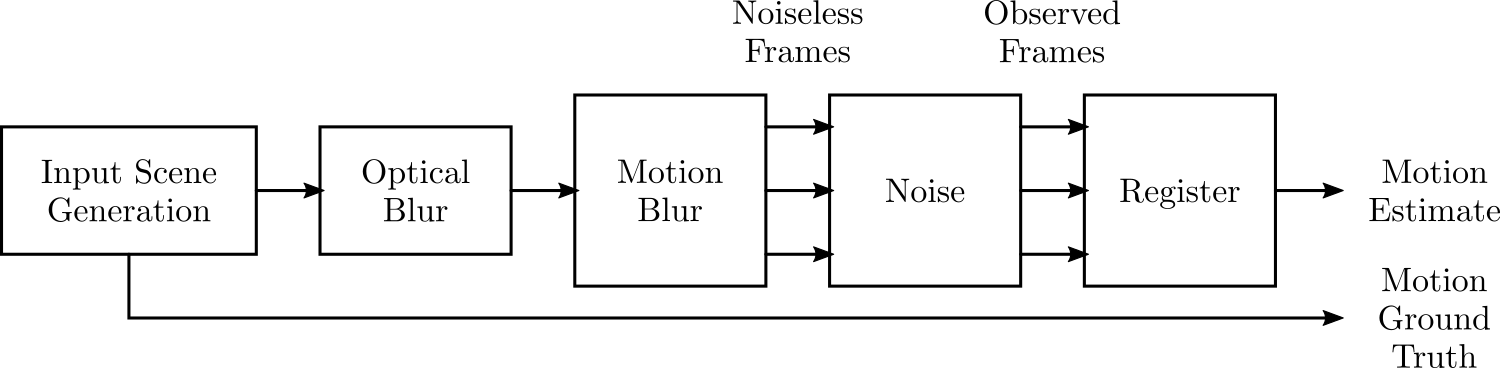
\includegraphics[width=1\textwidth]{figures/pipeline.png}
  \caption{Registration algorithm evaluation pipeline.}
  \label{fig:pipeline}
\end{figure}

\subsection{Input Scene Generation - Simplified Nanoflare Model} \label{sec:scene_nanoflare}

VISORS team member Klimchuk has studied coronal loops extensively and has used a hydrodynamical model called Enthalpy-based Thermal Evolution of Loops (EBTEL) to create a video of a changing scene containing many loops on a small patch of the Sun \cite{klimchuk2008}.  Within this small patch, nanoflares appear as superposed wide stripes across the entire scene which fade in and out at various inclinations and positions.

Instead of using the EBTEL frames directly, I use a custom Python function which generates frames that visually approximate the EBTEL frames, but at any field of view and resolution.  A comparison of an EBTEL frame and the Python approximation is given in Figure \ref{fig:strands}.  Additionally, any dynamic evolution of the nanoflares is ignored, as the total change expected over VISORS 10 second exposure is expected to be minimal, as shown in Figure \ref{fig:strands_static}.  More detail is given about VISORS exposure time and shutter speed in section \ref{sec:motion}

\begin{figure}
  \centering
  \begin{minipage}{.5\textwidth}
    \centering
    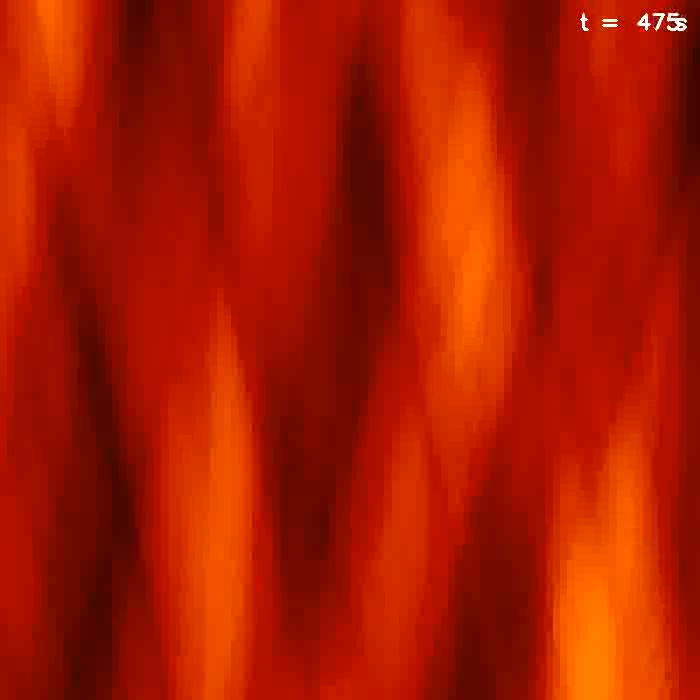
\includegraphics[width=.8\linewidth]{figures/strands_klimchuk.png}
  \end{minipage}%
  \begin{minipage}{.5\textwidth}
    \centering
    
\includegraphics[width=.8\linewidth]{figures/strands_mas.png}
  \end{minipage}
  \caption{Simulated field of views from EBTEL-generated video sequence and our Python approximation, respectively.  Field of view corresponds to square patch on Sun with sides about 2000km.}
  \label{fig:strands}
\end{figure}

\begin{figure}
  \centering
  \begin{minipage}{.5\textwidth}
    \centering
    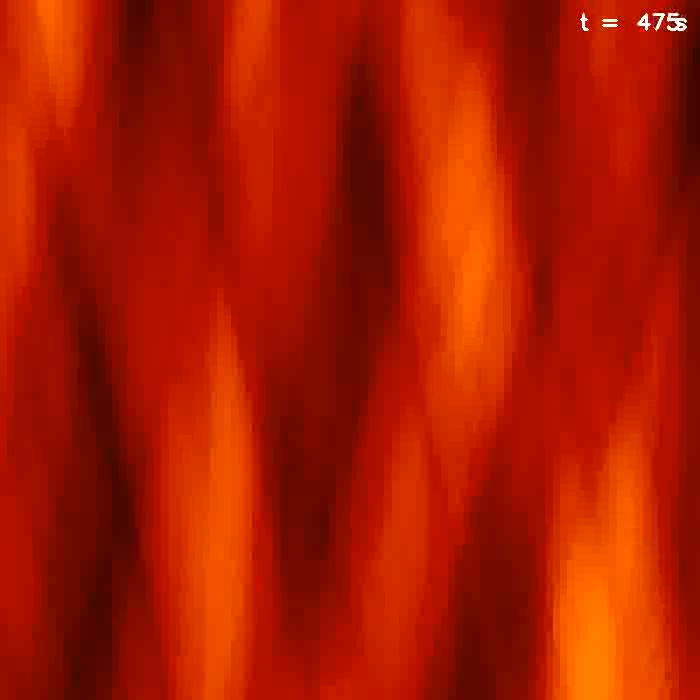
\includegraphics[width=.8\linewidth]{figures/strands_klimchuk.png}
  \end{minipage}%
  \begin{minipage}{.5\textwidth}
    \centering
    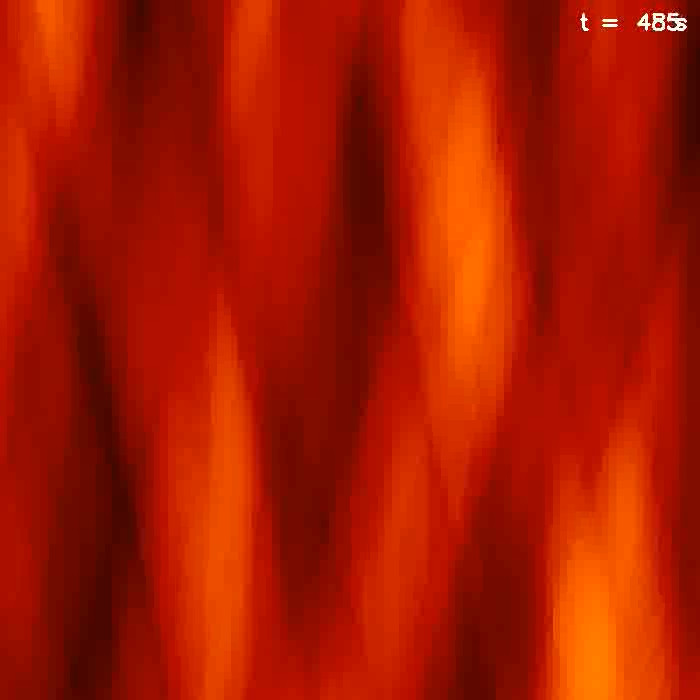
\includegraphics[width=.8\linewidth]{figures/strands_klimchuk2.png}
  \end{minipage}
  \caption{Two frames from EBTEL video separated by 10 s.  Very little evolution occurs over such a short window, which justifies the use of a static scene for simulation purposes.}
  \label{fig:strands_static}
\end{figure}

\subsection{Input Scene Generation - AIA Upsampled Data Model} \label{sec:scene_aia}

The accuracy of registration algorithms is dependent on the frequency content of the images being registered, so the presence or absence of nanoflares in the observed data is an important consideration in the simulation pipeline.  In order to establish worst-case bounds on the registration accuracy, it is possible to use lower-resolution measurements from previous missions with artifical fine structure added and evaluate the effect on the registration accuracy.

The Solar Dynamics Observatory (SDO) is one such mission with a resolution of 600 mas on its Atmospheric Imaging Assembly (AIA) instrument \cite{sdo}.  The AIA captures images of the full photosphere at many wavelengths, including several in the EUV spectrum.

I use the angular resolutions and detector sizes of VISORS and AIA (summarized in Table \ref{tab:params}) to compute the FOV of VISORS within the AIA image as 90 pixels in Equation \ref{eq:fov}, then upsample to the VISORS detector size of 750 pixels.  Finally, I artifically add small scale structure of size 2 pixels, computed in Equation \ref{eq:nanoflare}.  This process is illustrated in Figure \ref{fig:aia_modulated}.

%% \begin{gather*}
%%   600 \text{mas} - \text{AIA resolution} \\
%%   72 \text{mas} - \text{VISORS resolution} \\
%%   150 \text{mas} - \text{Nanoflare angular size} \\
%% \end{gather*}

\begin{gather}
  \svar{upsample factor} = r_{aia} / r_{visors} = 8.33 \notag \\
  \svar{FOV size} = N_{visors} / \svar{upsample factor} = 90 \text{ pixels} \label{eq:fov} \\
  \svar{Nanoflare size} = \svar{Nanoflare angular size} / r_{visors} = 2.08 \text{ pixels} \label{eq:nanoflare}
\end{gather}

\begin{figure}
  \centering
  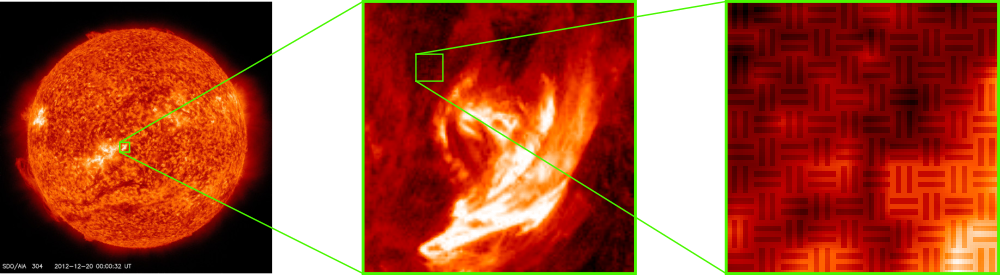
\includegraphics[width=1\textwidth]{figures/aia_modulated.png}
  \caption{Full photosphere capture from AIA, cropped region corresponding to input scene, and zoomed view showing synthetic modulated structure.}
  \label{fig:aia_modulated}
\end{figure}

Now that we have two models for generating input scenes, I will now describe steps which simulate physical distortions as the scene propagates through space and the imaging instrument.

\begin{table}
  \begin{center}
    \begin{tabular}{|c|c|c|}
      \hline
      \multicolumn{3}{|c|}{Sensor Parameters} \\
      \hline
      $r_{visors}$ & 72 mas & VISORS angular resolution \\
      $r_{aia}$ & 600 mas & AIA angular resolution \\
      $N_{aia}$ & 750 pixels & VISORS detector width \\
      \hline
      %% \multicolumn{3}{|c|}{VISORS Parameters} \\
      %% \hline
    \end{tabular}
    \caption{AIA and VISORS detector parameters}
    \label{tab:params}
  \end{center}
\end{table}

\subsection{Input Scene Scaling}

The input scenes generated thus far have dimensionless intensities ranging from 0 to 255.  In later sections, especially the noise analysis in Section \ref{sec:noise}, it is important that the intensities of the simulated observed frames are realistic as this has a direct impact on the level of detail visible and thus registration accuracy. 

The VISORS detector spacecraft carries a complementary metal-oxide semiconductor (CMOS) sensor which is sensitive to photons emitted by the solar photosphere.  Due to the discrete nature of light, a countable number of photons will impinge upon each pixel on the detector within a given window.  Since the integration time $T$ is known, the measured intensity is usually given as photons/s/pixel, which describes the average number of photons detected by a pixel per second.

VISORS team member Daw performed an analysis of multiple years of image data from AIA (shown in Figure \ref{fig:daw}) and determined both the average and maximum photon arrival rates of bright regions on the photosphere, accounting for the smaller size of VISORS pixels and losses due to VISORS optical path.  These computed values are shown in Table \ref{tab:daw}.

\begin{figure}
  \centering
  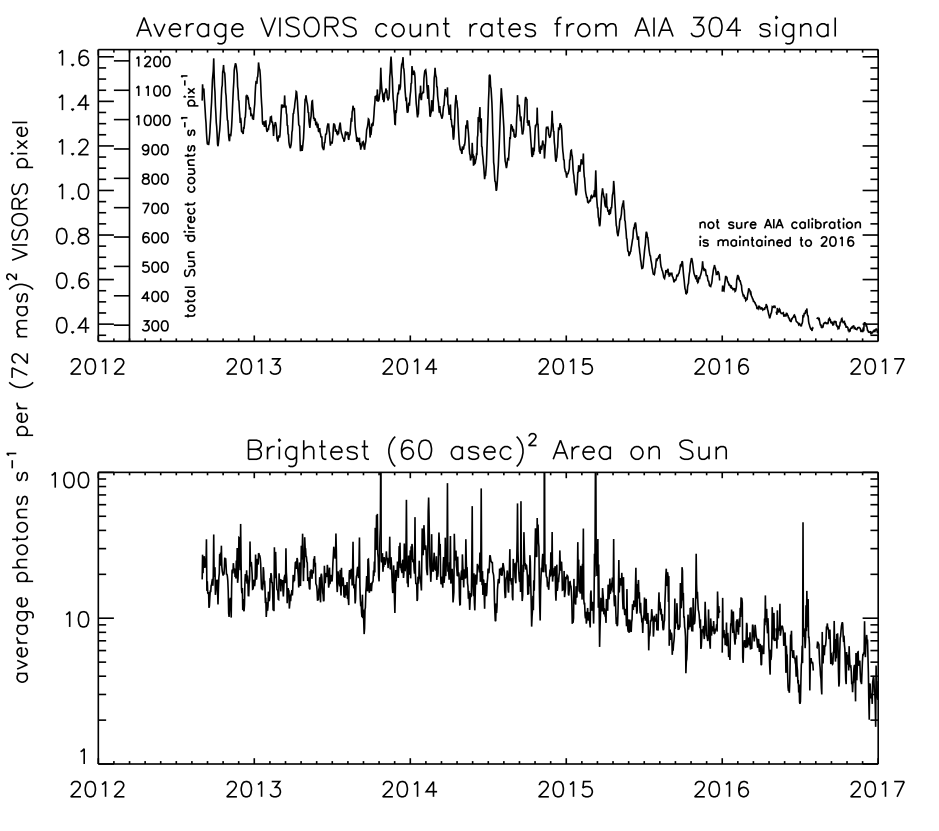
\includegraphics[width=0.8\textwidth]{figures/daw.png}
  \caption{Multi-year analysis of AIA photon arrival rates.}
  \label{fig:daw}
\end{figure}

\begin{table}
  \begin{center}
    \begin{tabular}{|c|c|c|}
      \hline
      \multicolumn{3}{|c|}{Expected VISORS photon rates} \\
      \hline
      $a_{mean}$ & 1.2 photons/s/pixel & average photon rate \\
      $a_{max}$ & 20 photons/s/pixel  & photon rate for brightest pixel \\
      \hline
      %% \multicolumn{3}{|c|}{VISORS Parameters} \\
      %% \hline
    \end{tabular}
    \caption{Expected photon rates in VISORS mission for 60 arcsecond FOV pointed at brightest active solar regions.}
    \label{tab:daw}
  \end{center}
\end{table}

In order to scale the unitless generated scenes to have a intensities measured in photons/s/pixel with the desired average $a_{avg}$ and maximum $a_{max}$ photon arrival rates, I use the affine mapping

$$ \left(a_{max} - \text{avg}(I)\right) \frac{I - \text{avg}(I)}{\max I - \text{avg}(I)} + a_{avg}\rightarrow I $$
where $I$ is the simulated input scene and $\rightarrow$ is an assignment operator.

\subsection{Optical Propagation}

In the VISORS project, light propagates from the Sun to the optics spacecraft, where it is diffracted by the photon sieve and again propagates to the sensor within the detector spacecraft.  This has the effect of slightly blurring the input scene even when the optics and detector spacecraft are in perfect focus.  An exact simulation of this process is intractible as it would require propagation of each pixel within the input scene through each hole in the photon sieve and propagation through free space to the detector.  Oktem et. al \cite{oktem2018} use the Fresnel approximation to obtain a closed form expression which relates the input scene to the image observed at the sensor in the detector spacecraft.  The transfer function is given terms of simple functions requiring no numerical integration techniques.

%% $$\tilde{h}_{sieve}(\omega_x, \omega_y) = \tilde{h}_0(\omega_x, \omega_y) + \sum_{m \text{ odd}} \tilde{h}_m(\omega_x, \omega_y)$$

%% where

\begin{align*}
  \tilde{h}_{sieve}(\omega_x, \omega_y) &=
  \frac{(\lambda d_i)^4}{2} e^{i \pi \Delta \lambda d_i^2 (\omega_x^2 + \omega_y^2)} \text{circ}\left(\frac{\lambda d_i}{D}\omega_x, \frac{\lambda d_i}{D} \omega_y \right) \\
  &+ \frac{(-1)}{\pi} (\lambda d_i)^4 \text{circ}\left(\frac{\lambda d_i}{D}\omega_x, \frac{\lambda d_i}{D} \omega_y \right)
  %% \Delta = 1/d_i + 1/d_s \\
  %% \epsilon_m = 1/d_i + 1/d_s - 1/f_m
\end{align*}
where

$$\Delta = 1/d_i + 1/d_s$$

$\omega_x$ and $\omega_y$ represent spatial frequency of the transfer function, $d_i$ the distance from the photon sieve to the image plane, $d_s$ the distance from the photon sieve to the source plane, $\lambda$ the wavelength of the incoming light, and $\text{circ}$ is a 2D unit circular aperture function.  The numerical values for sieve parameters are given in Table \ref{tab:sieve_params}.

This transfer function can be easily computed numerically and transformed into a point spread function (PSF) like the one shown in Figure \ref{fig:psf}, which can be convolved with the input scene to model optical path blurring.  Since we want to measure at point at which the image is in focus, the distance to the image plane should be equal to the focal length so that

$$d_i = f = \frac{Dw}{\lambda}$$

Now the transfer function can be computed and applied to the input scene using

$$I \ast h_{sieve} \rightarrow I$$
where $I$ is the input scene and $h_{sieve}$ is the inverse Fourier transform of the transfer function $\tilde{h}_{sieve}$.

The effect of this optical blur is shown in Figure \ref{fig:aia_blur} on a zoomed patch of the AIA input scene.  The synthetically added nanoflare modulation pattern is visibly degraded after the blurring kernel has been applied.

\begin{table}
  \begin{center}
    \begin{tabular}{|c|c|c|}
      \hline
      \multicolumn{3}{|c|}{VISORS Photon Sieve Parameters} \\
      \hline
      $\lambda$ & 30.4 nm & source wavelength \\
      $w$ & 17 $\mu$ m & sieve smallest hole diameter \\
      $D$ & 75 mm  & sieve diameter \\
      $d_s$ & $147.5 \cdot 10^6$ km  & distance to sun \\
      \hline
      %% \multicolumn{3}{|c|}{VISORS Parameters} \\
      %% \hline
    \end{tabular}
    \caption{VISORS noise parameters.  Dark current and read noise are determined by the CMOS specifications, while background noise has been computed by modelling light leakage around optics spacecraft.}
    \label{tab:sieve_params}
  \end{center}
\end{table}

\begin{figure}
  \centering
  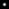
\includegraphics[width=0.3\textwidth]{figures/psf.png}
  \caption{Point spread function representing distortions due to VISORS optical path.}
  \label{fig:psf}
\end{figure}

\begin{figure}
  \centering
  \begin{minipage}{.5\textwidth}
    \centering
    
\includegraphics[width=0.8\textwidth]{figures/aia_modulate_zoom.png}
  \end{minipage}%
  \begin{minipage}{.5\textwidth}
    \centering
    
\includegraphics[width=0.8\textwidth]{figures/aia_modulate_zoom_blur.png}
  \end{minipage}
  \caption{Zoomed patch of AIA input scene before and after blurring by photon sieve point spread function.}
  \label{fig:aia_blur}
\end{figure}

\subsection{Motion Blurring} \label{sec:motion}

%% higher fidelity observation model for super resolution applications
%% extensible to other modes of integrated motion, such as rotation
%% elimination of edge artifacts

In order for the CMOS sensor on board the VISORS detector spacecraft to capture enough signal in these photons and overcome various sources of noise described in Section \ref{sec:noise}, it is necessary to hold the shutter open on the order of 1-10 seconds.  During this period, solar features within the VISORS FOV will have drifted significantly, causing motion-induced blurring and further degrading the captured frames.  From navigational requirements established by team member Koenig \cite{koenig}, at a 4 Hz capture rate solar features can be blurred by over 3 pixels \footnote{(0.2 mm/s drift) / (14 micron CMOS pixel pitch) / 4 Hz = 3.57 pixels}, corresponding to an angular resolution of 216 mas.  Being able to simulate the effects that frame integration time and spacecraft drift have on the observed frames is therefore extremely valuable both for evaluting performance of the registration algorithm and further constraining mission design parameters of the detector.

To simulate motion blur effects, I use the concept of a high-resolution grid described in Section \ref{sec:subpixel} where the pixel pitch of the observed frames is less than the pixel pitch of the underlying ground truth image.  In this thesis, the ratio of the high-resolution grid pitch and detector pixel pitch is $d=2$, shown in Figure \ref{fig:frame_integration}.

First, I compute the path taken during each frame by multiplying the drift rate $\bm{c}$ and total experiment duration, then dividing this line into $K$ segments of equal length.  Since this path is expressed in continuous coordinates, it must be discretized to the high-resolution grid.  This is achieved using Bresenham's line algorithm, which approximates a straight line drawn on a grid \cite{bresenham}.  The algorithm result and subdivided line are illustrated in Figure \ref{fig:bresenham}.

After the FOV path for each frame is calculated, the FOV is simply integrated for each pixel in each frame to get the observed frame, as shown in Figure \ref{fig:frame_subpixel}.  This is summarized mathematically as

\begin{equation}
  i_k[\bm{x}] = \frac{T}{|B_k(\bm{c})|} \sum_{\bm{x}_b \in B_k(\bm{c})} I[\bm{x} + \bm{x}_b]
\end{equation}
where $B_k(\bm{c})$ is the set of pixels offsets for the kth frame and a drift of $\bm{c}$ determined by Bresenham's algorithm.  In order to keep an image intensity which is physically meaningful (photons/s/pixel), the integrated frames are scaled by the frame integration period $T$ and divided by the number of summands in the path segment.

\begin{figure}
  \centering
  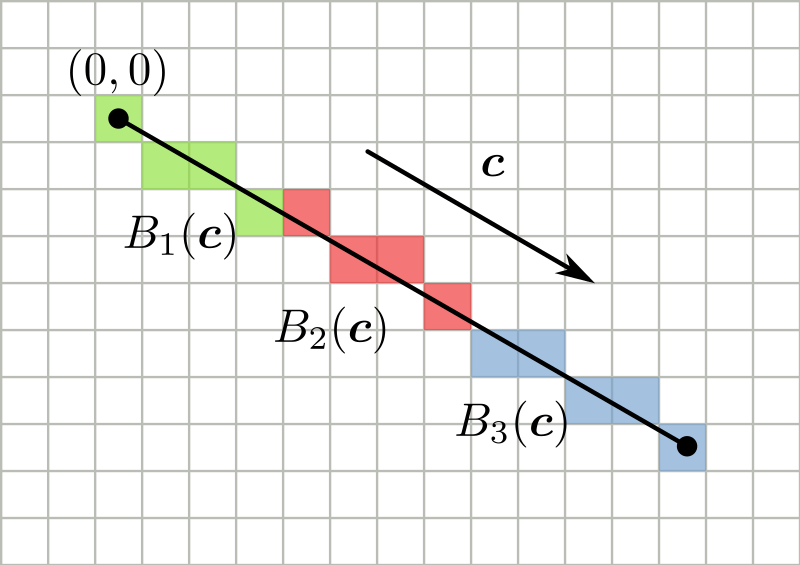
\includegraphics[width=0.6\textwidth]{figures/bresenham.png}
  \caption{Discrete path traced out by frames using Bresenham's line algorithm.}
  \label{fig:bresenham}
\end{figure}

\begin{figure}
  \centering
  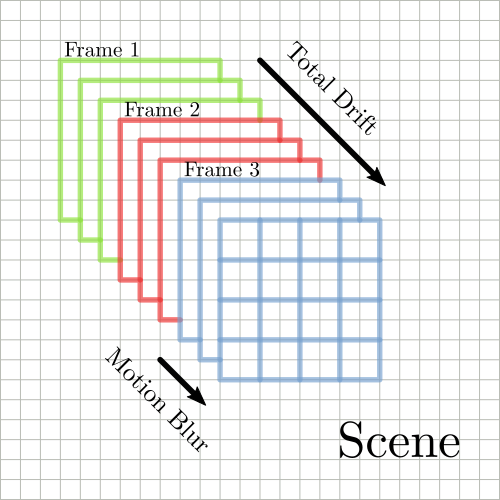
\includegraphics[width=0.6\textwidth]{figures/frame_integration.png}
  \caption{Frame integration of high-resolution grid under constant linear motion.}
  \label{fig:frame_subpixel}
\end{figure}

\begin{figure}
  \centering
  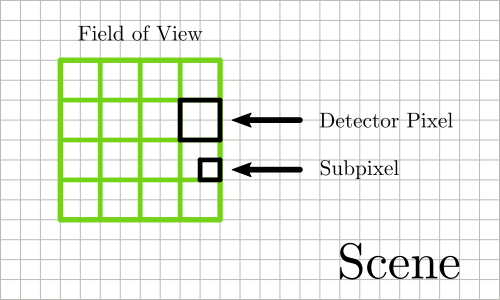
\includegraphics[width=0.6\textwidth]{figures/frame_subpixel.png}
  \caption{Detector instantaneous field of view and simulation high-resolution grid.}
  \label{fig:frame_integration}
\end{figure}

An alternative to the above strategy might have been to derive a blurring kernel to apply to all pixels in a cropped region of the input scene representing instantaneous position of the VISORS FOV.  This would be computed by convolving the FOV motion path within 1 frame with a unit function representing the size of a detector pixel on the high resolution grid to get an effective blurring kernel, as shown in Figure \ref{fig:effective_kernel}.  However, I chose the above technique for motion flexibiliity.

\begin{figure}
  \centering
  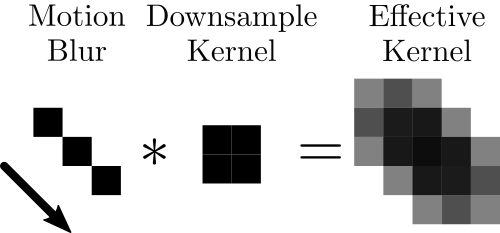
\includegraphics[width=0.4\textwidth]{figures/effective_kernel.png}
  \caption{Effective kernel due to motion and downsampling.}
  \label{fig:effective_kernel}
\end{figure}

%% First, a simple correlation of the effective kernel with the first FOV position of each frame would yield inaccurate measurements around the edge of each frame.  As shown in Figure \ref{fig:effective_problem}, there are pixel regions in the path of the sensor that have no representation in the observed frames.  This approximation may not have visible effects on a simple pixel level reconstruction, but can have significant impact on future super-resolution experiments where subpixel level details become significant.

In order for each pixel to have the same relative motion path, motion must be strictly translational.  Figure \ref{fig:effective_problem2} shows motion with a rotational component, where the shape of the path of each pixel is unique and the motion blurring is no longer spatially invariant.  While the multiframe registration method I propose models spacecraft motion as translational and linear, simulating motion blur in this way allows us to test motion model mismatch on the registration result.

%% \begin{figure}
%%   \centering
%%   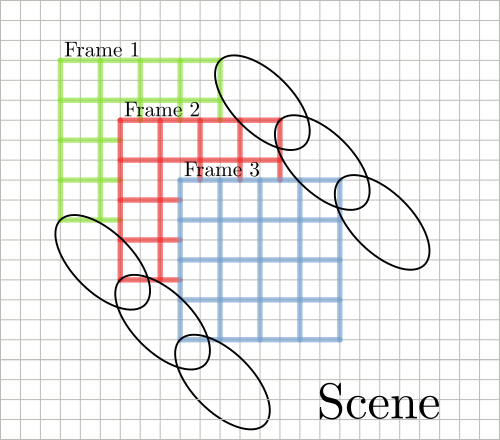
\includegraphics[width=0.6\textwidth]{figures/effective_problem.png}
%%   \caption{Circled: Pixel regions with no representation in observed frames when using simplified observation model.}
%%   \label{fig:effective_problem}
%% \end{figure}

\begin{figure}
  \centering
  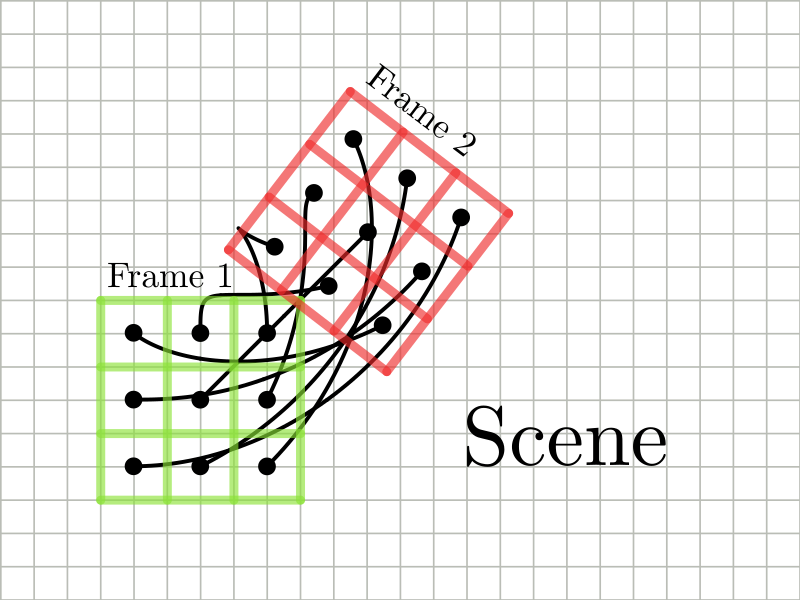
\includegraphics[width=0.6\textwidth]{figures/effective_problem2.png}
  \caption{Under non-translational motion, each detector pixel traces a unique path, so motion blurring is no longer spatially invariant.}
  \label{fig:effective_problem2}
\end{figure}

\begin{figure}
  \centering
  \begin{minipage}{.5\textwidth}
    \centering
    
\includegraphics[width=0.8\textwidth]{figures/aia_modulate_zoom_blur.png}
  \end{minipage}%
  \begin{minipage}{.5\textwidth}
    \centering
    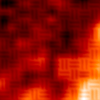
\includegraphics[width=0.8\textwidth]{figures/aia_modulate_zoom_blur_blur.png}
  \end{minipage}
  \caption{Zoomed patch of AIA input scene before and after motion-induced blurring.}
  \label{fig:aia_blur_blur}
\end{figure}

\subsection{Noise Sources} \label{sec:noise}

CMOS sensors are susceptible to several types of noise.  In this section, I model three types of noise.

The first source of noise is referred to as \emph{dark current noise}.  Dark current noise is created by random movement of charge within the sensor which falsely register as captured photons and is often caused by leakage current in the semiconductors used to fabricate the sensor \cite{dark}.  It is present even when no photons enter the detector (a dark field of view) and is characterized by the sensor manufacturer.  Dark noise is especially important to consider is low light conditions when the useful signal generated by impinging photons is overtaken by random signal generated by electrons.  Dark noise increases with increasing integration time.

Another source of noise is \emph{background noise} which is caused by light entering the detector from outside the optical path.  While this background light is caused by real photons hitting the detector, it is generally categorized as noise because these photons do not originate from the field of view being studied.  Background noise also increases with integration time.

These sources of noise are due to the quantum nature of energy and follow a Poisson process.  Together with the photons from the source itself they are referred to as \emph{shot noise} (though sometimes the photons coming from the source itself are named separately as \emph{photon shot noise}).

The final source of noise is \emph{read noise}, which occurs at the end of the frame integration interval.  Total accumulated charge is read from each pixel on the detector by an analog to digital converter (ADC).  Read noise is caused by interference from internal electronics and environmental sources and does not depend on integration time.

\begin{figure}
  \centering
  \begin{minipage}{.3\textwidth}
    \centering
    
\includegraphics[width=0.8\textwidth]{figures/aia_modulate_zoom_blur.png}
  \end{minipage}%
  \begin{minipage}{.3\textwidth}
    \centering
    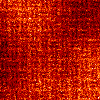
\includegraphics[width=0.8\textwidth]{figures/aia_modulate_zoom_blur_blur_p.png}
  \end{minipage}
  \begin{minipage}{.3\textwidth}
    \centering
    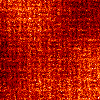
\includegraphics[width=0.8\textwidth]{figures/aia_modulate_zoom_blur_blur_pn.png}
  \end{minipage}
  \caption{Zoomed patch of observed frame with no noise, after shot noise, and after shot noise and read noise.}
  \label{fig:aia_blur_blur_pn}
\end{figure}

\begin{table}
  \begin{center}
    \begin{tabular}{|c|c|c|}
      \hline
      \multicolumn{3}{|c|}{VISORS noise parameters} \\
      \hline
      $n_d$ & 0.8 photons/s/pixel  & dark current noise \\
      $n_b$ & 2 photons/s/pixel & background noise \\
      $n_r$ & 1 photons/s/read  & read noise \\
      \hline
      %% \multicolumn{3}{|c|}{VISORS Parameters} \\
      %% \hline
    \end{tabular}
    \caption{VISORS noise parameters.  Dark current and read noise are determined by the CMOS specifications, while background noise has been computed by modelling light leakage around optics spacecraft.}
    \label{tab:daw}
  \end{center}
\end{table}

The observation model used for generating each observed noisy frame $i_k$ is

$$\mathcal{N}\Big( \text{Pois}(i_k + T (n_d + n_b)), \, n_r^2\Big) \rightarrow i_k$$

An example of a noisy observation frame after shot noise and read noise is shown in Figure \ref{fig:aia_blur_blur_pn}

\section{Registration Results} \label{sec:results}

In this section, I characterize the error in the registration algorithm by running it on simulated noisy frames generated by the forward model and computing the Euclidean distance between the estimated drift $\bm{\hat{c}}$ and actual drift $\bm{c}$.

$$\text{err} = \lVert \hat{\bm{c}} - \bm{c} \rVert_2$$

While error in the drift estimated by the registration algorithm can be used as a metric for algorithm performance, it is also informative to look at the reconstruction derived from this drift estimate.  I use a simple frame coadding technique to obtain a reconstruction.

$$I_{recon} = \sum_{k=1}^K i_k\left[\bm{x} - \text{round}(k \hat{\bm{c}})\right]$$

This method serves as a baseline only and can certainly be improved by techniques such as super-resolution, denoising, motion deblurring, and regularization.

In the rest of this section, I evaluate reconstruction performance under the two types of input scenes presented previously, investigate algorithm accuracy while varying noise levels and motion in a Monte Carlo simulation, and examine the effect on reconstructions when the constraint of constant translational motion between frames is relaxed.

Unless otherwise stated, experiments were performed with $T=0.25$, $K=40$, $a_{max} = 20$ and $\bm{c} = [.675,\, .675]$


\subsection{Input Scene Model}

In sections \ref{sec:scene_nanoflare} and \ref{sec:scene_aia}, I presented two methods for generating an input scene.  The first is based upon hydrodynamical simulations of nanoflare evolution and has been scaled to the expected nanoflare size.  The second is derived from low-resolution images from AIA which has been synthetically altered to add some fine-grained structure.

Figure \ref{fig:recon_nanoflare} is an illustration of a test with the nanoflare input scene that shows the ground truth, a single noisy frame out of a set of 40, and the coadded reconstruction after running the registration algorithm.  The algorithm was successful and the 40 input frames were registered and coadded to obtain a reconstruction which is much higher fidelity than any single frame.

Figure \ref{fig:recon_aia} is a similar test using an upsampled AIA input scene, but has a second row so that the synthetic structure is visible.  The results from this experiment are notable, because even though the fine synthetic structure is no longer visible in a single frame due to noise, the algorithm is able to successfully register the frames to sufficient accuracy so that these structures become visible again in the reconstruction.  The parameters used in these experiments are given in table \ref{tab:recon_params}.

\begin{figure}[h]
  \centering
  \begin{minipage}{.3\textwidth}
    \centering
    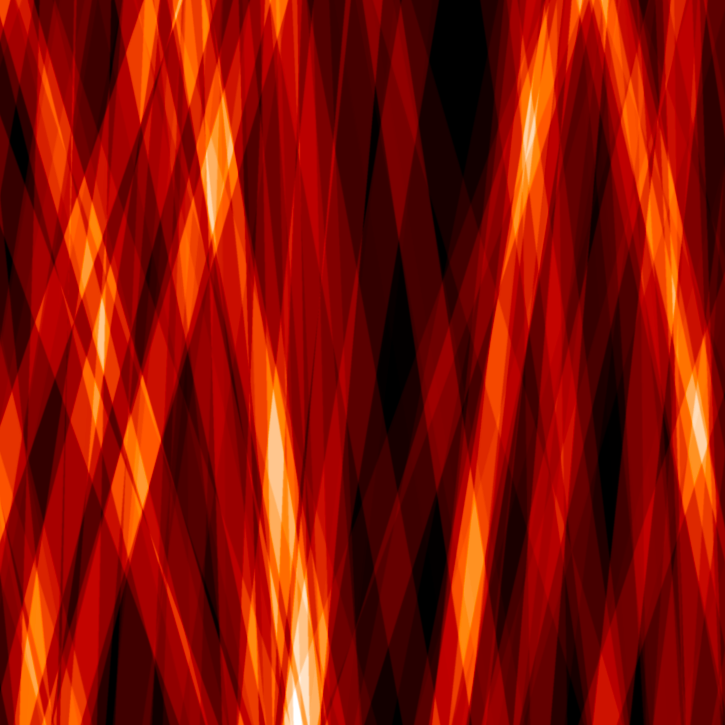
\includegraphics[width=1\textwidth]{figures/strands_truth.png}
  \end{minipage}
  \begin{minipage}{.3\textwidth}
    \centering
    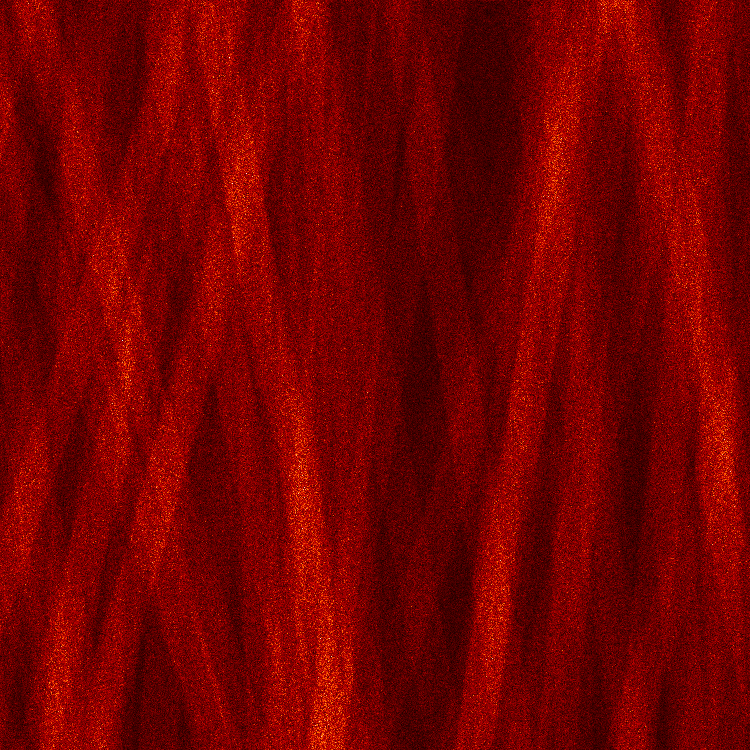
\includegraphics[width=1\textwidth]{figures/strands_frame.png}
  \end{minipage}
  \begin{minipage}{.3\textwidth}
    \centering
    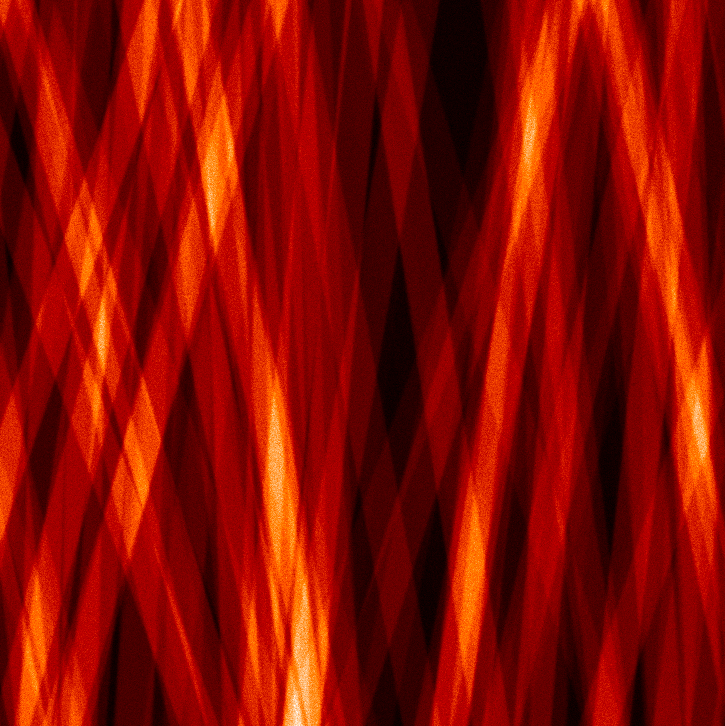
\includegraphics[width=1\textwidth]{figures/strands_recon.png}
  \end{minipage}
  \caption{Modulated nanoflare input scene, noised + blurred observation frame, coadded reconstruction.}
  \label{fig:recon_nanoflare}
\end{figure}

\begin{figure}[h]
  \centering
  \begin{minipage}{.3\textwidth}
    \centering
    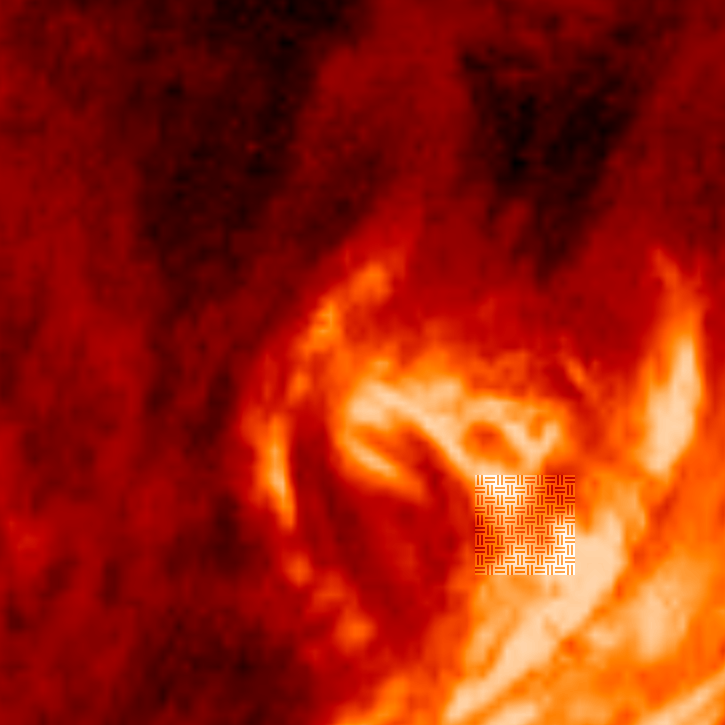
\includegraphics[width=1\textwidth]{figures/aia_truth.png}
  \end{minipage}
  \begin{minipage}{.3\textwidth}
    \centering
    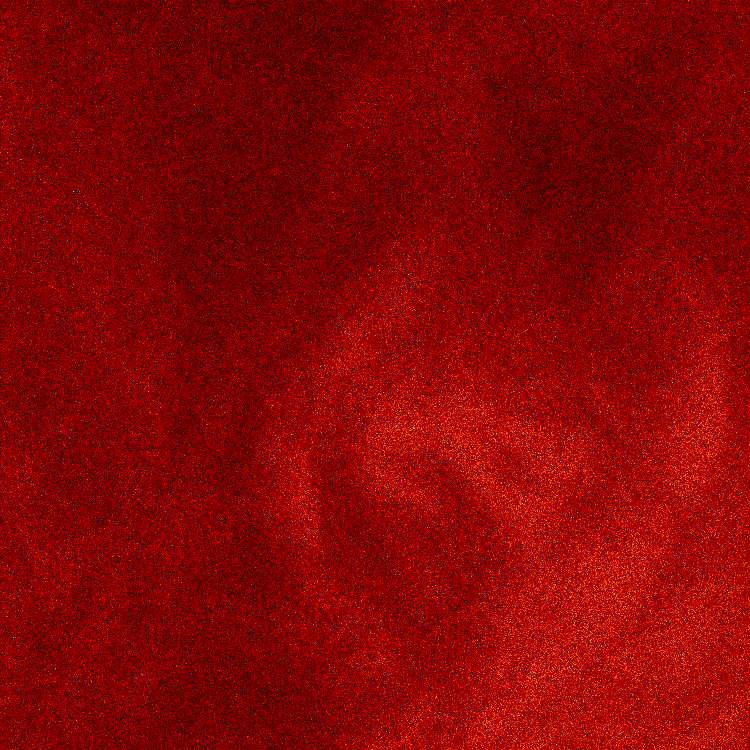
\includegraphics[width=1\textwidth]{figures/aia_frame.png}
  \end{minipage}
  \begin{minipage}{.3\textwidth}
    \centering
    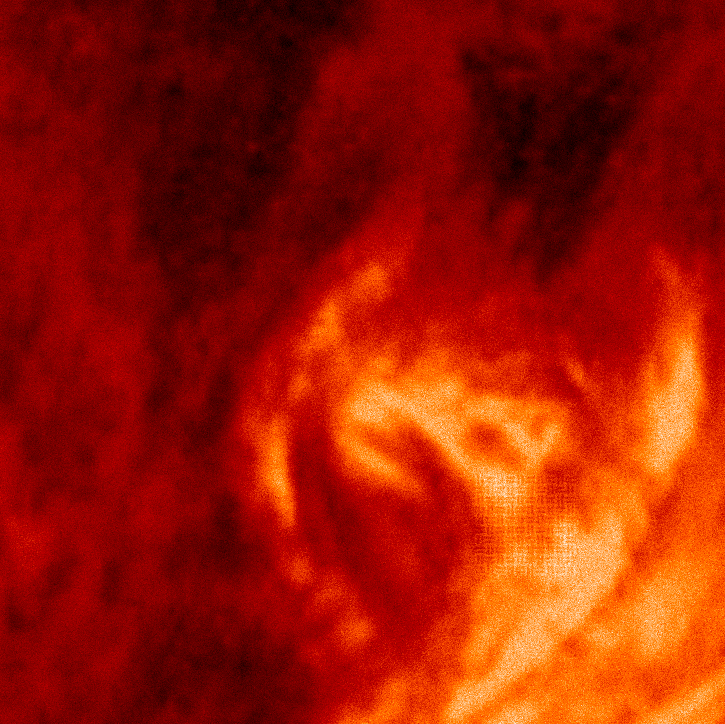
\includegraphics[width=1\textwidth]{figures/aia_recon.png}
  \end{minipage}
  \begin{minipage}{.3\textwidth}
    \centering
    
\includegraphics[width=1\textwidth]{figures/aia_truth_zoom.png}
  \end{minipage}
  \begin{minipage}{.3\textwidth}
    \centering
    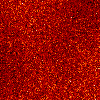
\includegraphics[width=1\textwidth]{figures/aia_frame_zoom.png}
  \end{minipage}
  \begin{minipage}{.3\textwidth}
    \centering
    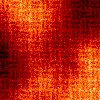
\includegraphics[width=1\textwidth]{figures/aia_recon_zoom.png}
  \end{minipage}
  \caption{Top row, from left: Modulated AIA input scene, noised + blurred observation frame, coadded reconstruction.  Bottom row, from left: Same as top row, but zoomed to show modulation detail.}
  \label{fig:recon_aia}
\end{figure}

\begin{table}
  \begin{center}
    \begin{tabular}{|c|c|c|}
      \hline
      \multicolumn{3}{|c|}{VISORS noise parameters} \\
      \hline
      $T$ & 0.25 s  & frame integration time \\
      $K$ & 40 frames & number of frames \\
      $a_{max}$ & 20 photons/s  & photon rate of brightest pixel \\
      $\bm{c}$ & [0.141,\,0.141] mm/s & interframe drift \\
      & [2.53,\,2.53] pixels/s & \\
      \hline
      %% \multicolumn{3}{|c|}{VISORS Parameters} \\
      %% \hline
    \end{tabular}
    \caption{VISORS noise parameters.  Dark current and read noise are determined by the CMOS specifications, while background noise has been computed by modelling light leakage around optics spacecraft.}
    \label{tab:recon_params}
  \end{center}
\end{table}


\subsection{Noise Variation}

Maximum photon count $a_{max}$ is a major contributor to shot noise in the observation model and dominates read noise as shown in Figure \ref{fig:aia_blur_blur_pn}.
The expected value of 20 photons/s/pixel for the maximum photon count in VISORS was derived by analyzing bright regions on the photosphere from many AIA images and compensating for differences in detector pixel size, quantum efficiency and efficiency of instrument optical paths.  However, this is a worse case estimate and in reality may be higher if small scale structures are observed.  In Figure \ref{fig:noise_tolerance}, I sweep the maximum photon count with several values around 20 to illustrate reconstruction quality at these other possible noise levels.  At 20 photon/s/pixel, fine structure is just barely visible in the reconstruction, and at 100 photons/s/pixel the modulated grid is quite clear.

\begin{figure}
  \centering
  \makebox[\textwidth][c]{
  \begin{minipage}{.19\textwidth}
    \centering
    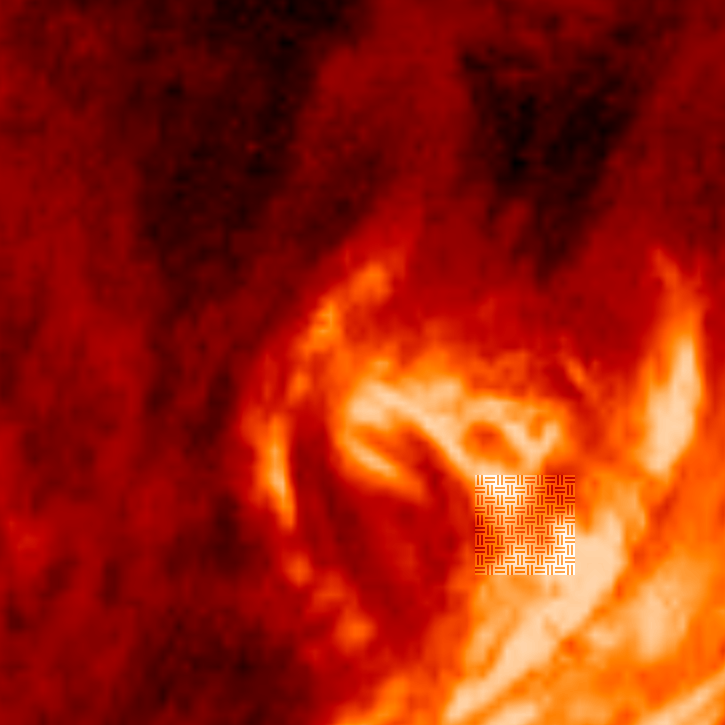
\includegraphics[width=.95\textwidth]{figures/aia_truth.png}
  \end{minipage}%
  \begin{minipage}{.19\textwidth}
    \centering
    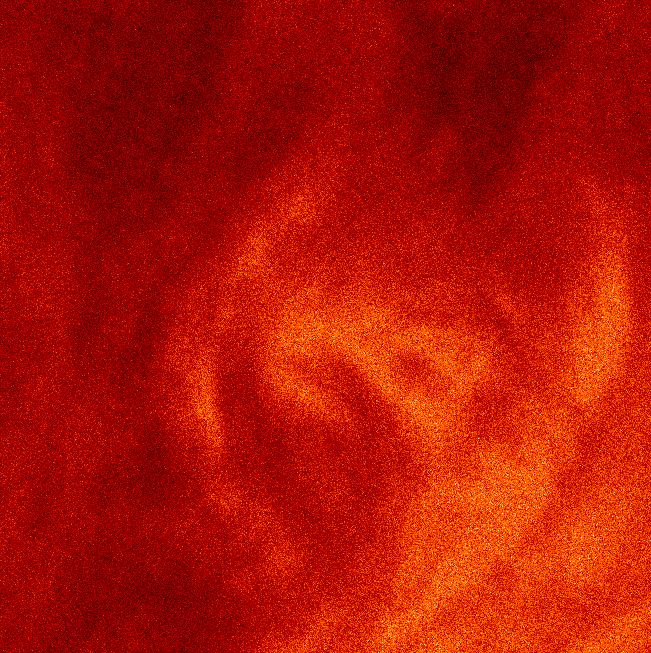
\includegraphics[width=.95\textwidth]{figures/aia_recon10.png}
  \end{minipage}%
  \begin{minipage}{.19\textwidth}
    \centering
    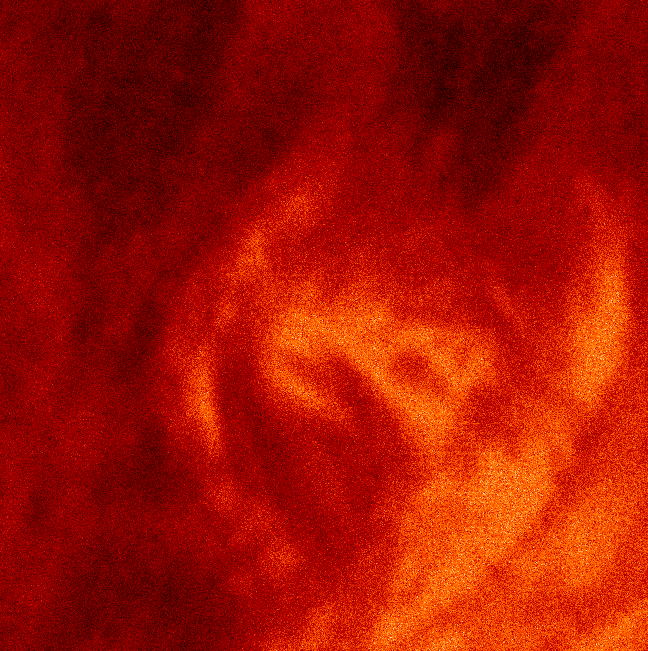
\includegraphics[width=.95\textwidth]{figures/aia_recon20.png}
  \end{minipage}%
  \begin{minipage}{.19\textwidth}
    \centering
    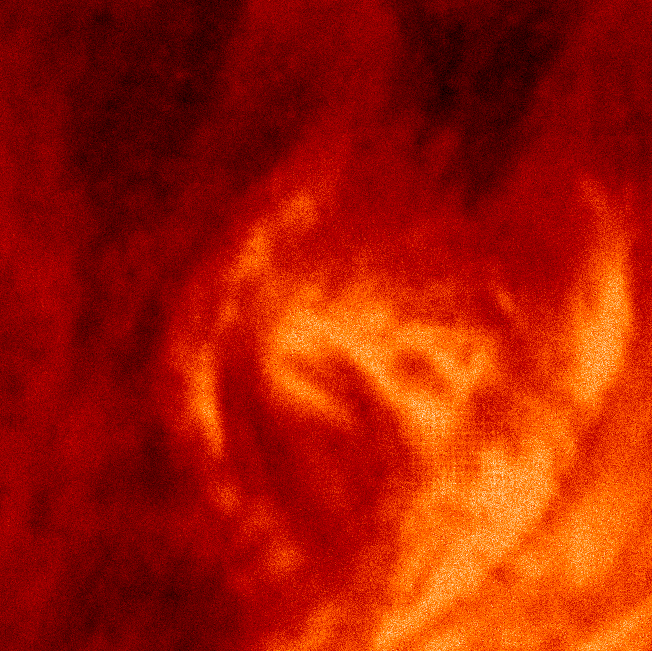
\includegraphics[width=.95\textwidth]{figures/aia_recon50.png}
  \end{minipage}%
  \begin{minipage}{.19\textwidth}
    \centering
    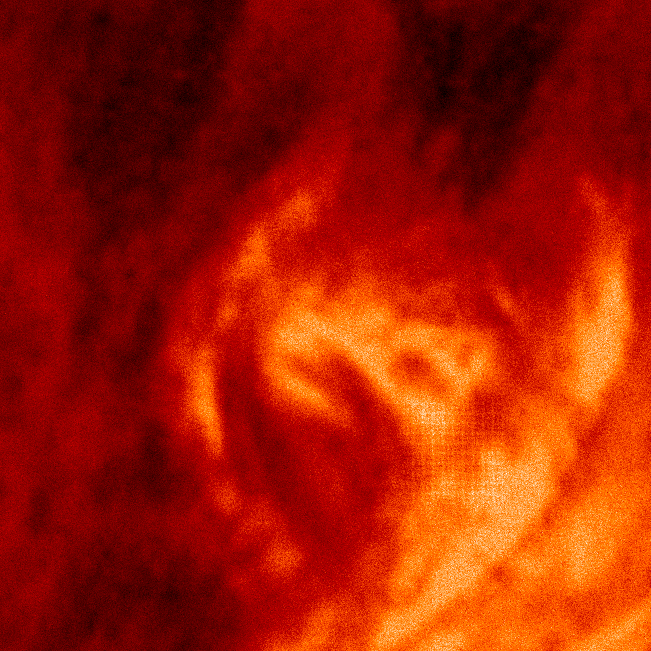
\includegraphics[width=.95\textwidth]{figures/aia_recon80.png}
  \end{minipage}%
  \begin{minipage}{.19\textwidth}
    \centering
    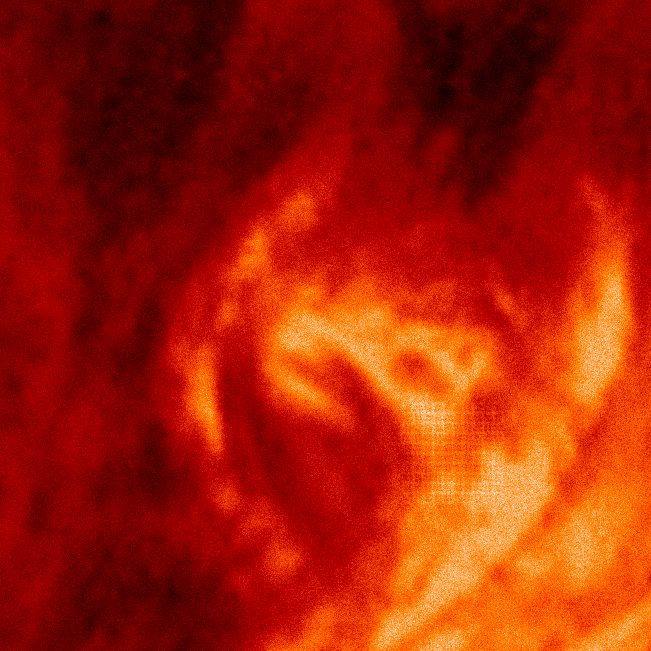
\includegraphics[width=.95\textwidth]{figures/aia_recon100.png}
  \end{minipage}%
  }
  \makebox[\textwidth][c]{
  \begin{minipage}{.19\textwidth}
    \centering
    
\includegraphics[width=.95\textwidth]{figures/aia_truth_zoom.png}
  \end{minipage}%
  \begin{minipage}{.19\textwidth}
    \centering
    \includegraphics[width=.95\textwidth]{figures/aia_recon_zoom10.png}
  \end{minipage}%
  \begin{minipage}{.19\textwidth}
    \centering
    \includegraphics[width=.95\textwidth]{figures/aia_recon_zoom20.png}
  \end{minipage}%
  \begin{minipage}{.19\textwidth}
    \centering
    \includegraphics[width=.95\textwidth]{figures/aia_recon_zoom50.png}
  \end{minipage}%
  \begin{minipage}{.19\textwidth}
    \centering
    \includegraphics[width=.95\textwidth]{figures/aia_recon_zoom80.png}
  \end{minipage}%
  \begin{minipage}{.19\textwidth}
    \centering
    \includegraphics[width=.95\textwidth]{figures/aia_recon_zoom100.png}
  \end{minipage}%
  }
  \caption{Top: AIA input scene ground truth, and reconstructions for input scaling ($a_{max}$) of 10, 20, 50, 80 and 100 photons/s/pixel.  Bottom: Same as Top, but zoomed to show modulation detail.}
  \label{fig:noise_tolerance}
\end{figure}


\subsection{Monte Carlo Simulation}

Other system parameters besides noise can affect the registration result, such as drift velocity and drift angle.

In Figure \ref{fig:monte}, I swept these three parameters across a range of realistic values and plotted the error in the drift estimate for each.  Additionally, I repeated each experiment 10 times in a Monte Carlo simulation to get an estimate of the mean and standard deviation of the error.  Several conclusions can be drawn from this plot.  First, mean estimation error decreases as noise decreasing (increasing $a_{max}$) and converges to a mean of around 0.05.  This number is corroborated by the reconstruction experiments in the previous section because an interframe drift estimate error of 0.05 corresponds to a total alignment error of $39 \times 0.05 \approx 1$ pixels between the first and last frames in the sequence, which is less than the nanoflare feature size of 2 pixels derived in section \ref{sec:scene_aia}.

Next, drift estimation error improves slightly with a decreasing drift velocity.  This is possibly due to a decrease in the amount of motion blur which preserves high frequency structure than the registration algorithm uses for accurate drift estimation.

Finally, the drift error is fairly independent of the angle of drift of the spacecraft.  This is expected for the modulated AIA scene which has approximately equal frequency content in both the x and y directions, but the algorithm may performly differently for different drift angles if this is not the case.

\begin{figure}
  \centering
  \makebox[\textwidth][c]{
    \includegraphics[width=1.25\textwidth]{figures/monte.png}
  }
  \caption{Monte Carlo simulation showing error in the drift estimate under varying drift rates, drift angles, and maximum photon counts ($a_{max}$). The solid line is the mean while the shaded region is $\pm 1$ standard deviation.}
  \label{fig:monte}
\end{figure}

\subsection{Motion Model Mismatch}

%% \section{Other Image Classes}
While the relative motion of solar features within VISORS field of view is expected to be constant and translational, it is useful to know the effect a violation of this motion model has on the registration result.  Here I adjust the simulations to include a constant roll on the boresight axis of the formation.  Tweaking the model given in Section \ref{sec:model}, we now have the more general coordinate transform relations

\begin{eqnarray}
  f_{j,k}(\bm{x}) = R_{\theta (k - j)}\left(\bm{x} - \bm{c}(k - j)\right) \\
  f_{j,k}(\bm{x}) = f_{l,m}(\bm{x})
  \label{eqn:constant}
\end{eqnarray}

for $j,k,l,m \in 1, ..., K$ when $k - j = m - l$.  $\theta$ is the roll rate of the formation.

\begin{figure}
  \centering
  \makebox[\textwidth][c]{
  \begin{minipage}{.19\textwidth}
    \centering
    \includegraphics[width=.95\textwidth]{figures/aia_truth_zoom.png}
  \end{minipage}%
  \begin{minipage}{.19\textwidth}
    \centering
    \includegraphics[width=.95\textwidth]{figures/aia_recon_zoom5.png}
  \end{minipage}%
  \begin{minipage}{.19\textwidth}
    \centering
    \includegraphics[width=.95\textwidth]{figures/aia_recon_zoom10.png}
  \end{minipage}%
  \begin{minipage}{.19\textwidth}
    \centering
    \includegraphics[width=.95\textwidth]{figures/aia_recon_zoom20.png}
  \end{minipage}%
  \begin{minipage}{.19\textwidth}
    \centering
    \includegraphics[width=.95\textwidth]{figures/aia_recon_zoom40.png}
  \end{minipage}%
  \begin{minipage}{.19\textwidth}
    \centering
    \includegraphics[width=.95\textwidth]{figures/aia_recon_zoom60.png}
  \end{minipage}%
  }
  \caption{Zoomed reconstructions from upsampled AIA scene under different rates of roll $\theta$.}
  \label{fig:mismatch}
\end{figure}

Figure \ref{fig:mismatch} shows zoomed patches from reconstructions of the upsampled AIA scene under several rates of roll.  As $\theta$ is increased, misalignment which cannot be accounted for by shifting and coadding dominates and the fine scale structure is no longer visible.  The formation roll rate should be constrained to be below this threshold to successfully image such fine structures.


\chapter{Conclusion} \label{chap:conclusion}

This chapter is a summary of the work presented in this thesis and describes potential future work.

\section{Registration Algorithm and Forward Model}

In the first chapter of this thesis, I introduced the VISORS project and the problem of image registration.  I detailed several types of coordinate transforms that may be used in image registration and explained why a simple translational model is appropriate for the VISORS project.  In chapter \ref{chap:preliminaries}, I described a framework for categorizing image registration methods and illustrated several algorithms capable of registering two frames, as well as algorithms capable of registering images on a subpixel level.  In the next chapter, I introduced the problem of multiframe image registration and related it to the two-frame problem with a mathematical model.  I then described a new parameterless, non-iterative multiframe registration method which should have more robust performance than a simple extension of a two-frame method to multiple frames.  I showed that this method is similar from the ML solution when the drift between frames is assumed to be constant and linear.

\section{Forward Model and Registration Results}

In section \ref{sec:pipeline}, I began describing a forward optical pipeline which simulates frames captured by VISORS starting from generating photosphere scenes to capture by the detector.  The first step of this pipeline was the generation of the solar scene using a physics based model, and another more conservative model based on data from previous orbiters.  Next, these scenes were scaled from dimensionless images to a map of photon arrival rates, then propagated through the VISORS optical system.  These propagated scenes were then motion blurred using a method which is more sophisticated than global convolution which can account for spatially variant blurring in the case of complex spacecraft motion.  Finally, I applied a noise which models sensor read out noise and various types of shot noise.

In section \ref{sec:results}, I performed an array of numerical experiments which illustrate the performance of the multiframe registration algorithm.  I showed that images can be recovered even when no structure is clearly visible in individual observation frames, and specifically that fine-grained structure in the modulated nanoflare scene is preserved given a sufficiently high SNR.  Furthermore, I ran Monte Carlo simulations to characterize the mean and standard deviation of the error in the algorithm's drift estimate.  Finally, I showed that small amounts of model mismatch in the form of a rotational component in the coordinate transform model can be tolerated by the algorithm.

\section{Future Work}

The primary goal of this thesis was to develop a registration algorithm for the purposes of determining the presence of small scale nanoflares within the VISORS observations.  As a result, I elected to use a relative simple reconstruction scheme via coadding of the observed frames using the registration algorithm's estimate of interframe drift.  As a result, there is much room for improvement in which can boost the quality of the reconstructions.

The motion blur introduced in section \ref{sec:pipeline} is not accounted for during reconstruction.  There are many motion deblurring algorithms available, from methods removing simple Gaussian blurring to more sophisticated methods that can account for complex motion all of which should sharpen the reconstructions.  Furthermore, the motion blurring kernel can be computed from the final drift estimate, which means that non-blind deblurring methods may be used.

Finally, super-resolution techniques may be applied which may reveal more fine structures within the reconstruction.  Many super-resolution methods depend on accurate image registration either as an initialization step or use the registration algorithm in an iterative fashion.  The registration algorithm proposed in this thesis could be substituted into these super-resolution techniques.

%% - regularization, motion deblurring, super resolution more sophisticated than simple coadding scheme

%%%%%%%%%%%%%%%%%%%%%%%%%%%%%%%%%%%%%%%%%%%%%%%%%%%%%%%%%%%%%%%%%%%%%%%%%%%%%%%
% APPENDIX
%
\appendix
%\include{apx}

\backmatter

%%%%%%%%%%%%%%%%%%%%%%%%%%%%%%%%%%%%%%%%%%%%%%%%%%%%%%%%%%%%%%%%%%%%%%%%%%%%%%%
% BIBLIOGRAPHY
%
\bibliographystyle{IEEE_ECE}
% Put references in BibTeX format in thesisrefs.bib.
\bibliography{thesisrefs}

\end{document}
\endinput
